%Modified for DBS by Paul Laird

% *******************************  Thesis Template **************************
% Please have a look at the README.md file for info on how to use the template

\documentclass[a4paper,12pt,times,numbered,print,index,custombib]{Classes/PhDThesisPSnPDF}
\newcommand\posscite[1]{\citeauthor{#1}'s (\citeyear{#1})}



% ******************************************************************************
% ******************************* Class Options ********************************
% *********************** See README for more details **************************
% ******************************************************************************

% `a4paper'(The University of Cambridge PhD thesis guidelines recommends a page
% size a4 - default option) or `a5paper': A5 Paper size is also allowed as per
% the Cambridge University Engineering Deparment guidelines for PhD thesis
%
% `11pt' or `12pt'(default): Font Size 10pt is NOT recommended by the University
% guidelines
%
% `oneside' or `twoside'(default): Printing double side (twoside) or single
% side.
%
% `print': Use `print' for print version with appropriate margins and page
% layout. Leaving the options field blank will activate Online version.
%
% `index': For index at the end of the thesis
%
% `draftclassic': For draft mode without loading any images (same as draft in book)
%
% `draft': Special draft mode with line numbers, images, and water mark with
% timestamp and custom text. Position of the text can also be modified.
%
% `abstract': To generate only the title page and abstract page with
% dissertation title and name, to submit to the Student Registry
%
% `chapter`: This option enables only the specified chapter and it's references
%  Useful for review and corrections.
%
% ************************* Custom Page Margins ********************************
%
% `custommargin`: Use `custommargin' in options to activate custom page margins,
% which can be defined in the preamble.tex. Custom margin will override
% print/online margin setup.
%
% *********************** Choosing the Fonts in Class Options ******************
%
% `times' : Times font with math support. (The Cambridge University guidelines
% recommend using times)
%
% `fourier': Utopia Font with Fourier Math font (Font has to be installed)
%            It's a free font.
%
% `customfont': Use `customfont' option in the document class and load the
% package in the preamble.tex
%
% default or leave empty: `Latin Modern' font will be loaded.
%
% ********************** Choosing the Bibliography style ***********************
%
% `authoryear': For author-year citation eg., Krishna (2013)
%
% `numbered': (Default Option) For numbered and sorted citation e.g., [1,5,2]
%
% `custombib': Define your own bibliography style in the `preamble.tex' file.
%              `\RequirePackage[square, sort, numbers, authoryear]{natbib}'.
%              This can be also used to load biblatex instead of natbib
%              (See Preamble)
%
% **************************** Choosing the Page Style *************************
%
% `default (leave empty)': For Page Numbers in Header (Left Even, Right Odd) and
% Chapter Name in Header (Right Even) and Section Name (Left Odd). Blank Footer.
%
% `PageStyleI': Chapter Name next & Page Number on Even Side (Left Even).
% Section Name & Page Number in Header on Odd Side (Right Odd). Footer is empty.
%
% `PageStyleII': Chapter Name on Even Side (Left Even) in Header. Section Number
% and Section Name in Header on Odd Side (Right Odd). Page numbering in footer

% Uncomment to change page style
%\pagestyle{PageStyleII}

% ********************************** Preamble **********************************
% Preamble: Contains packages and user-defined commands and settings
% ******************************************************************************
% ****************************** Custom Margin *********************************

% Add `custommargin' in the document class options to use this section
% Set {innerside margin / outerside margin / topmargin / bottom margin}  and
% other page dimensions
\ifsetCustomMargin
  \RequirePackage[left=37mm,right=30mm,top=35mm,bottom=30mm]{geometry}
  \setFancyHdr % To apply fancy header after geometry package is loaded
\fi

% Add spaces between paragraphs
%\setlength{\parskip}{0.5em}
% Ragged bottom avoids extra whitespaces between paragraphs
\raggedbottom
% To remove the excess top spacing for enumeration, list and description
%\usepackage{enumitem}
%\setlist[enumerate,itemize,description]{topsep=0em}

% *****************************************************************************
% ******************* Fonts (like different typewriter fonts etc.)*************

% Add `customfont' in the document class option to use this section

\ifsetCustomFont
  % Set your custom font here and use `customfont' in options. Leave empty to
  % load computer modern font (default LaTeX font).
  %\RequirePackage{helvet}

  % For use with XeLaTeX
  %  \setmainfont[
  %    Path              = ./libertine/opentype/,
  %    Extension         = .otf,
  %    UprightFont = LinLibertine_R,
  %    BoldFont = LinLibertine_RZ, % Linux Libertine O Regular Semibold
  %    ItalicFont = LinLibertine_RI,
  %    BoldItalicFont = LinLibertine_RZI, % Linux Libertine O Regular Semibold Italic
  %  ]
  %  {libertine}
  %  % load font from system font
  %  \newfontfamily\libertinesystemfont{Linux Libertine O}
\fi

% *****************************************************************************
% **************************** Custom Packages ********************************

% ************************* Algorithms and Pseudocode **************************

%\usepackage{algpseudocode}


% ********************Captions and Hyperreferencing / URL **********************

% Captions: This makes captions of figures use a boldfaced small font.
%\RequirePackage[small,bf]{caption}

\RequirePackage[labelsep=space,tableposition=top]{caption}
\renewcommand{\figurename}{Fig.} %to support older versions of captions.sty


% *************************** Graphics and figures *****************************

%\usepackage{rotating}
%\usepackage{wrapfig}

% Uncomment the following two lines to force Latex to place the figure.
% Use [H] when including graphics. Note 'H' instead of 'h'
%\usepackage{float}
%\restylefloat{figure}

% Subcaption package is also available in the sty folder you can use that by
% uncommenting the following line
% This is for people stuck with older versions of texlive
%\usepackage{sty/caption/subcaption

\usepackage{subcaption}
\usepackage[T1]{fontenc}
\usepackage[utf8]{inputenc}
\usepackage{authblk}

% ********************************** Tables ************************************
\usepackage{booktabs} % For professional looking tables
\usepackage{multirow}

%\usepackage{multicol}
%\usepackage{longtable}
%\usepackage{tabularx}
\bibliographystyle{unsrtnat}
\usepackage[numbers,sort&compress]{natbib}

% *********************************** SI Units *********************************
\usepackage{siunitx} % use this package module for SI units


% ******************************* Line Spacing *********************************

% Choose linespacing as appropriate. Default is one-half line spacing as per the
% University guidelines

% \doublespacing
% \onehalfspacing
% \singlespacing


% ************************ Formatting / Footnote *******************************

% Don't break enumeration (etc.) across pages in an ugly manner (default 10000)
%\clubpenalty=500
%\widowpenalty=500

%\usepackage[perpage]{footmisc} %Range of footnote options


% *****************************************************************************
% *************************** Bibliography  and References ********************

%\usepackage{cleveref} %Referencing without need to explicitly state fig /table

% Add `custombib' in the document class option to use this section
\usepackage[authoryear]{natbib}
%  \ifuseCustomBib
%     \RequirePackage[sort, authoryear]{natbib} % CustomBib

% If you would like to use biblatex for your reference management, as opposed to the default `natbibpackage` pass the option `custombib` in the document class. Comment out the previous line to make sure you don't load the natbib package. Uncomment the following lines and specify the location of references.bib file

%\RequirePackage[backend=biber, style=numeric-comp, citestyle=numeric, sorting=nty, natbib=true]{biblatex}
%\bibliography{References/references} %Location of references.bib only for biblatex

%\fi

% changes the default name `Bibliography` -> `References'
\renewcommand{\bibname}{References}


% ******************************************************************************
% ************************* User Defined Commands ******************************
% ******************************************************************************

% *********** To change the name of Table of Contents / LOF and LOT ************

%\renewcommand{\contentsname}{My Table of Contents}
%\renewcommand{\listfigurename}{My List of Figures}
%\renewcommand{\listtablename}{My List of Tables}


% ********************** TOC depth and numbering depth *************************

\setcounter{secnumdepth}{2}
\setcounter{tocdepth}{1}


% ******************************* Nomenclature *********************************

% To change the name of the Nomenclature section, uncomment the following line

%\renewcommand{\nomname}{Symbols}


% ********************************* Appendix ***********************************

% The default value of both \appendixtocname and \appendixpagename is `Appendices'. These names can all be changed via:

%\renewcommand{\appendixtocname}{List of appendices}
%\renewcommand{\appendixname}{Appndx}

% *********************** Configure Draft Mode **********************************

% Uncomment to disable figures in `draft'
%\setkeys{Gin}{draft=true}  % set draft to false to enable figures in `draft'

% These options are active only during the draft mode
% Default text is "Draft"
%\SetDraftText{DRAFT}

% Default Watermark location is top. Location (top/bottom)
%\SetDraftWMPosition{bottom}

% Draft Version - default is v1.0
%\SetDraftVersion{v1.1}

% Draft Text grayscale value (should be between 0-black and 1-white)
% Default value is 0.75
%\SetDraftGrayScale{0.8}


% ******************************** Todo Notes **********************************
%% Uncomment the following lines to have todonotes.

%\ifsetDraft
%	\usepackage[colorinlistoftodos]{todonotes}
%	\newcommand{\mynote}[1]{\todo[author=kks32,size=\small,inline,color=green!40]{#1}}
%\else
%	\newcommand{\mynote}[1]{}
%	\newcommand{\listoftodos}{}
%\fi

% Example todo: \mynote{Hey! I have a note}

\usepackage{float}
\usepackage{siunitx}
\usepackage{hyperref}
\usepackage{booktabs}
\usepackage[normalem]{ulem}
\useunder{\uline}{\ul}{}

% ************************ Thesis Information & Meta-data **********************
% Thesis title and author information, refernce file for biblatex
% ************************ Thesis Information & Meta-data **********************
%% The title of the thesis
\title{Writing your thesis in \texorpdfstring{\\ \LaTeX2e}{LaTeX2e}}
%\texorpdfstring is used for PDF metadata. Usage:
%\texorpdfstring{LaTeX_Version}{PDF Version (non-latex)} eg.,
%\texorpdfstring{$sigma$}{sigma}

%% Subtitle (Optional)
%\subtitle{Using the CUED template}

%% The full name of the author
\author{DIT Student}

%% Department (eg. Department of Engineering, Maths, Physics)
%\dept{Department of Engineering}

%% University and Crest
\university{Dublin Institute of Technology}
% Crest minimum should be 30mm.
\crest{
\includegraphics[width=0.4\textwidth]{DIT}}
%% Use this crest, if you are using the college crest
%% Crest long miminum should be 65mm
%\crest{
\includegraphics[width=0.45\textwidth]{University_Crest_Long}}

%% College shield [optional] 
% Crest minimum should be 30mm.
%\collegeshield{
\includegraphics[width=0.2\textwidth]{CollegeShields/Kings}}


%% Supervisor (optional)
%% for multiple supervisors, append each supervisor with the \newline command
%\supervisor{Prof. A.B. Supervisor\newline
%Prof. C.D. Supervisor}

%% Supervisor Role (optional) - Supervisor (default) or advisor
% \supervisorrole{\textbf{Supervisors: }}
%% if no title is desired:
% \supervisorrole{}

%% Supervisor line width: required to align supervisors
%\supervisorlinewidth{0.35\textwidth}

%% Advisor (optional)
%% for multiple advisors, append each advisor with the \newline command
%\advisor{Dr. A. Advisor\newline
%Dr. B. Advisor}
     
%% Advisor Role (optional) - Advisor (default) or leave empty
% \advisorrole{Advisors: }
%% if no title is required
% \advisorrole{}

%% Advisor line width: required to align supervisors
%\advisorlinewidth{0.25\textwidth}


%% You can redefine the submission text:
% Default as per the University guidelines:
% ``This dissertation is submitted for the degree of''
%\renewcommand{\submissiontext}{change the default text here if needed}

%% Full title of the Degree
\degreetitle{Bachelor of Science}

%% College affiliation (optional)
%\college{King's College}

%% Submission date
% Default is set as {\monthname[\the\month]\space\the\year}
%\degreedate{September 2014} 

%% Meta information
\subject{LaTeX} \keywords{{LaTeX} {Thesis}}


% ***************************** Abstract Separate ******************************
% To printout only the titlepage and the abstract with the PhD title and the
% author name for submission to the Student Registry, use the `abstract' option in
% the document class.

\ifdefineAbstract
 \pagestyle{empty}
 \includeonly{Declaration/declaration, Abstract/abstract}
\fi

% ***************************** Chapter Mode ***********************************
% The chapter mode allows user to only print particular chapters with references
% Title, Contents, Frontmatter are disabled by default
% Useful option to review a particular chapter or to send it to supervisior.
% To use choose `chapter' option in the document class

\ifdefineChapter
 \includeonly{Chapter3/chapter3}
\fi

% ******************************** Front Matter ********************************
\begin{document}

\frontmatter

\begin{titlepage}
    \begin{center}
            
        \Huge
        \textbf{UNIVERSITY OF TRENTO}
            
        \vspace{0.5cm}
        \LARGE
            Department of Sociology and Social Research
        
        \vspace{0.5cm}
        \large
           Master's Degree \\ in  \\ Data Science
            
        \vspace{1cm}
         
        
\includegraphics[width=0.4\textwidth]{logos/images.png}   
       
       
        \vspace{0.5cm}
        \LARGE
            \textbf{Analyzing Polarization in Climate Change Tweets during COP: A Multi-Layer Networks and Topic Modeling Approach}
            
        \vspace{0.5cm}
            
        
     \end{center}  
     
\raggedright

\large
    Thesis by:
    \vspace{0.2cm}\author[3]\textbf{Alessio Gandelli}

    
\raggedleft

\large
    Supervisor:
    \vspace{0.3cm}\author[1]\textbf{Elena Pavan\thanks{elena.pavan@unitn.it}}\\ 
\large
    Co-Supervisor.
    \vspace{0.3cm}\author[2]\textbf{Matteo Magnani\thanks{matteo.magnani@it.uu.se}}\\


    
  


\begin{center}
    \vspace{2cm}
        Academic year 2021/2023
\end{center}
    
\end{titlepage}


%% ******************************* Thesis Dedidcation ********************************

\begin{dedication} 

I would like to dedicate this thesis to \dots

\end{dedication}
%% ******************************* Thesis Declaration ***************************

\begin{declaration}

I hereby declare that the work described in this dissertation is, except where otherwise stated, entirely my own work and has not been submitted as an exercise for a degree at this or any other University.

% Author and date will be inserted automatically from thesis.tex \author \degreedate

\end{declaration}
% ************************** Thesis Acknowledgements **************************

\begin{acknowledgements}      


And I would like to acknowledge ...


\end{acknowledgements}

% ************************** Thesis Abstract *****************************
% Use `abstract' as an option in the document class to print only the titlepage and the abstract.
\begin{abstract}
This thesis aimed to investigate the polarization of users in the climate change discussion surrounding the Conferences of Parties, with a specific focus on the 26th Conference. Unlike previous studies, this research adopted a topic-by-topic approach using a multi-layer network framework. The objectives were twofold: first, to identify the most polarized topics of COP26 and compare them with a longitudinal study involving COP21; and second, to explore user polarization across different topics and investigate whether users engaging in more topics exhibit higher levels of polarization. 
The findings revealed that in the most polarized topics, there was an almost equal distribution of users on both sides, indicating a sharp divide in opinions. Notably, this polarization was particularly evident in the Canadian discussion on limiting the use of coal and oil, as well as the air travel debate. Additionally, it was observed that the Canadian discussion on Fossil Fuel was not consistently polarized, as it exhibited complete non-polarization during COP21, confirming the results obtained by other researches.
Furthermore, users tended to remain aligned with a specific side of the discussion across multiple topics, although there was no correlation between the number of topics and the polarization score.
\end{abstract}


% *********************** Adding TOC and List of Figures ***********************

\tableofcontents

\listoffigures

\listoftables

% \printnomenclature[space] space can be set as 2em between symbol and description
%\printnomenclature[3em]

%\printnomenclature

% ******************************** Main Matter *********************************
\mainmatter

%!TEX root = ../thesis.tex
%*******************************************************************************
%*********************************** First Chapter *****************************
%*******************************************************************************

\chapter{Introduction}  %Title of the First Chapter

\ifpdf
    \graphicspath{{Chapter1/Figs/Raster/}{Chapter1/Figs/PDF/}{Chapter1/Figs/}}
\else
    \graphicspath{{Chapter1/Figs/Vector/}{Chapter1/Figs/}}
\fi
\section{Background}
Climate change is a well known problem among scientist since longtime but only in the past few years has become mainstream, in part thanks to Greta Thunberg and Fridays for Future people were more aware of the problem. As we can see in Fig \ref{fig:google_greta} only after 2019 people started searching ( and talking) about a climate crisis, underlining  the urgency with which we should act. It is also true that the strikes   caused inconvenience to many normal citizen trying to go to their workplace. This mean that someone may have developed a bad feeling towards this activism and thus towards climate change.
\\

Usually when people wants to complain about something they write on Twitter  where breaking down geographical barriers you can get in touch with thousands of people that agree with you. This may cause polarization and echo chambers.

\begin{figure}
    \centering
    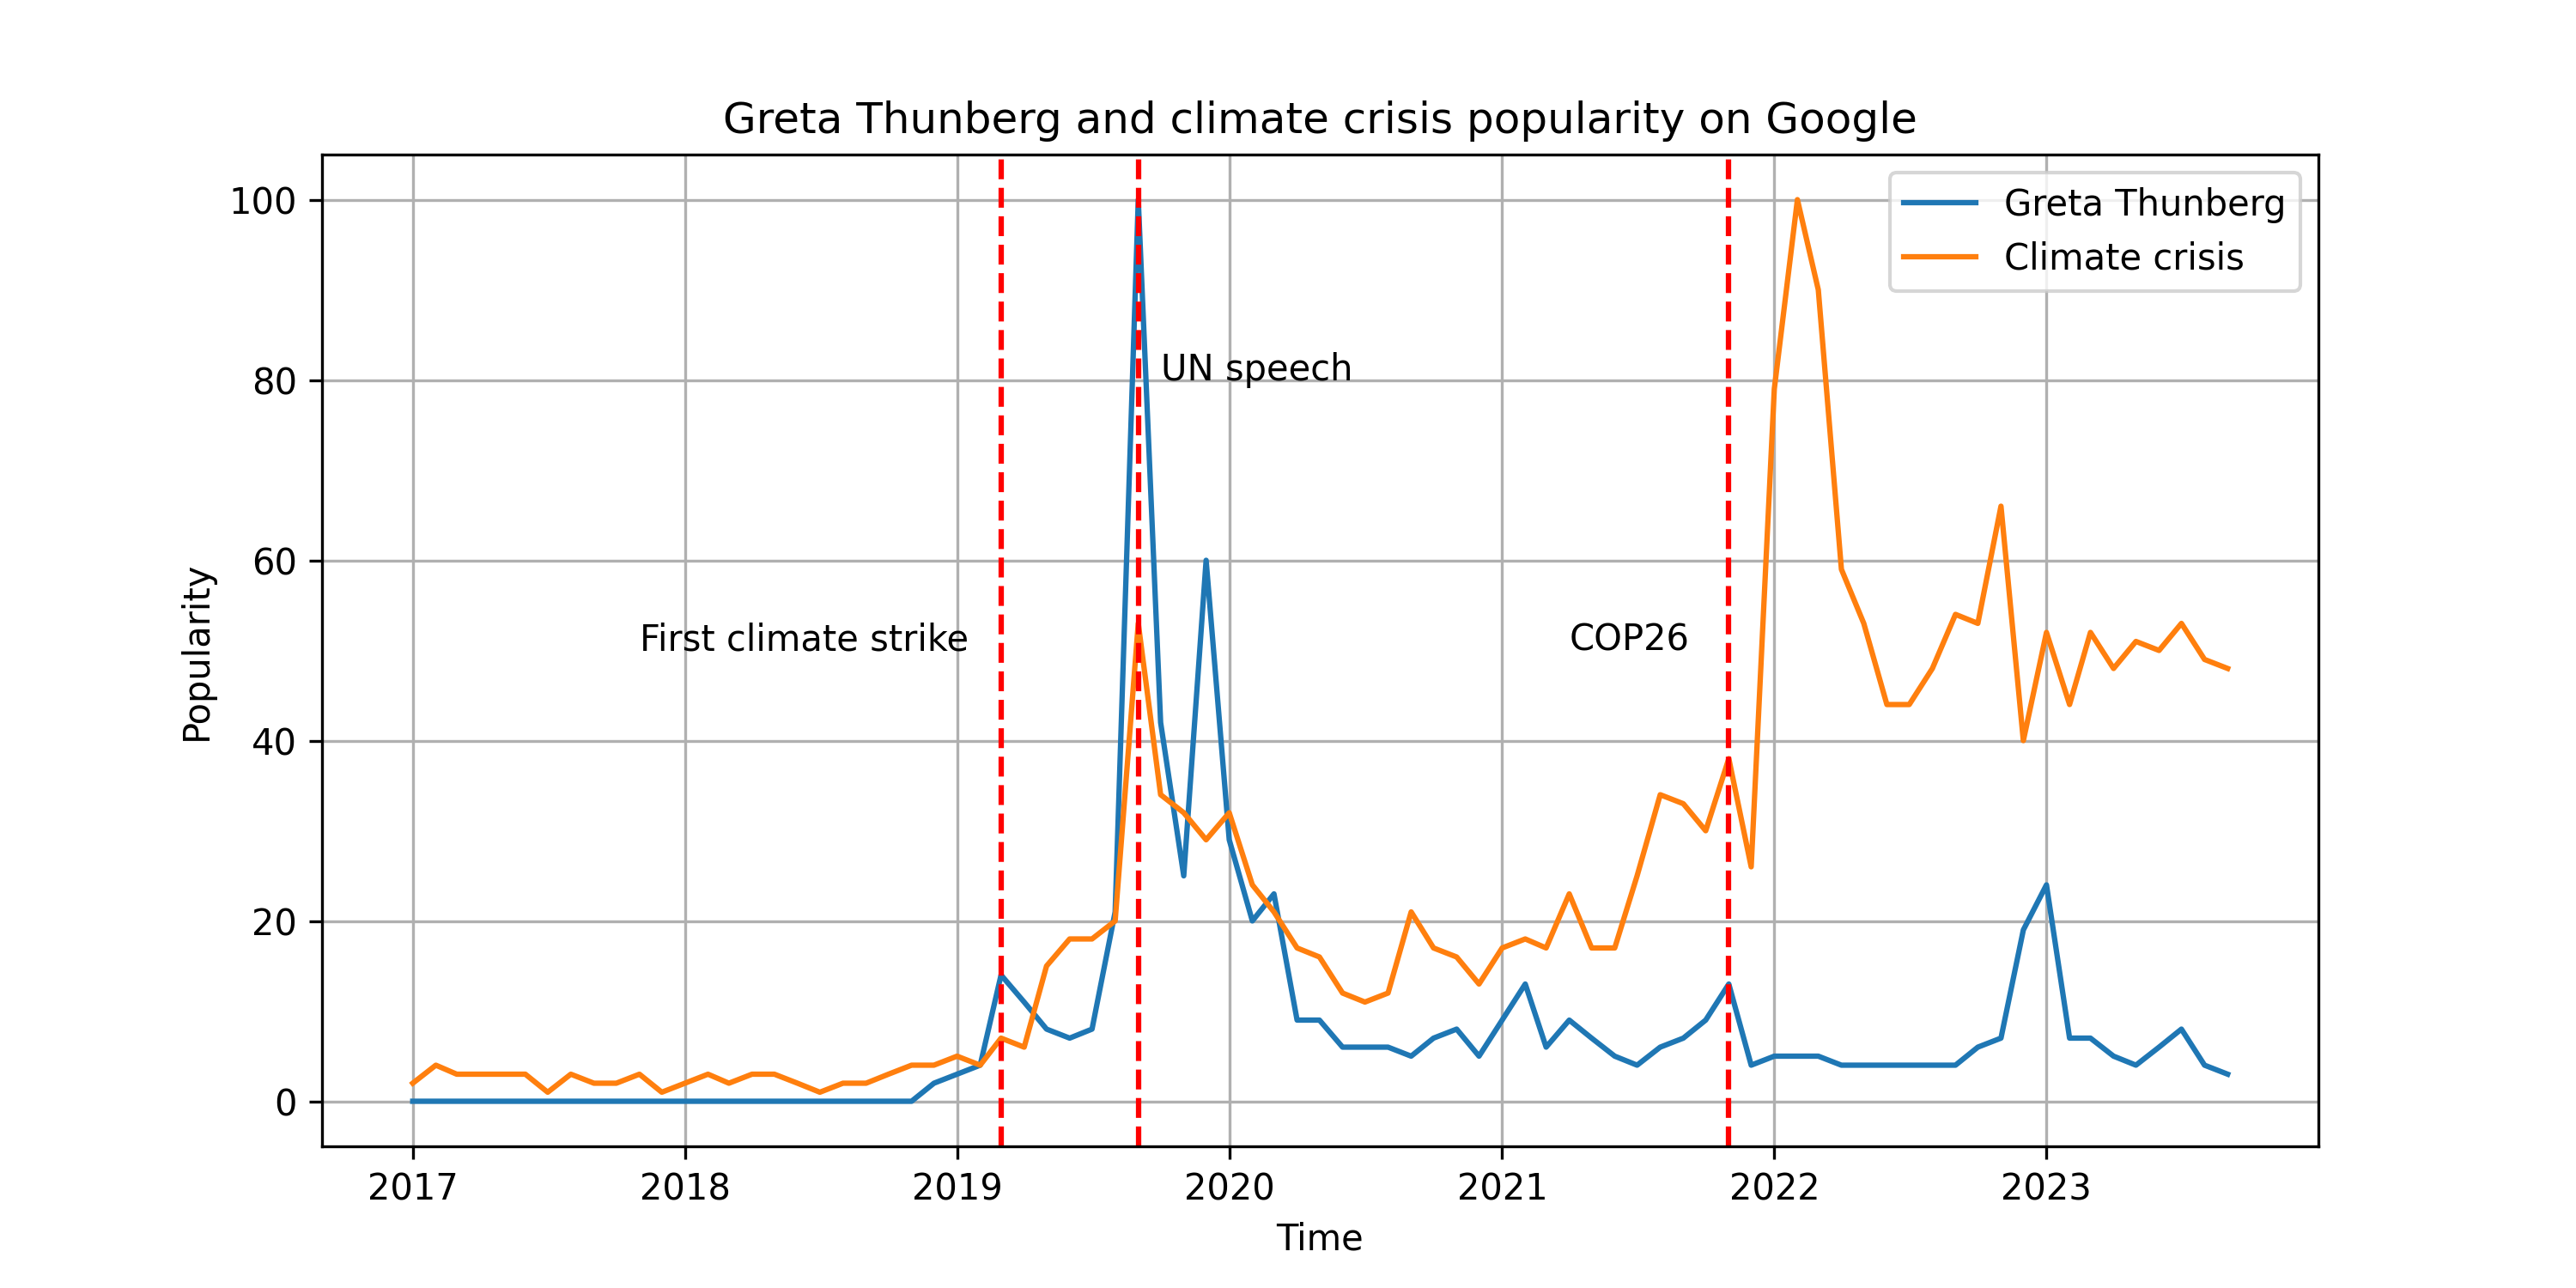
\includegraphics[width=0.85\linewidth]{Chapter1/figures/greta_climate_crisis.png}
    \caption{Interest on google over the time of Greta Thunberg and climat crisis}
    \label{fig:google_greta}
\end{figure}
In particular twitter is a place where political debate take place, and political events like 
Conference of Parties (COP) are the perfect joint between these two worlds because are the conferences where the highest political figures of many countries meet and talk about the climate emergencies. 



\paragraph{Conference of Parties}
Conferences of Parties are yearly conferences organized by United Nations where the topic of discussion is climate change, the first has been held in 1995 in Berlin, the most relevant are:
\begin{itemize}
    \item \textbf{COP3}: Kyoto protocol (1997)
    \item \textbf{COP21}: Paris agreement (2015)
    \item \textbf{COP26}: Glasgow Climate Pact (2021)
\end{itemize}

\\

For the first one unfortunatly we do not have twitter data but for the latter two we have, and our focus will be on that two .

In particular we will study the well known phenomenon among social scientist of polarization i.e. the tendency to choose one side of the political spectrum and stick with all their believes without trying to go outside their echo chamber.\\




This work lays its foundations on the research of Falkenberg et al \cite{falkenberg_growing_2022} where they discovered that the cop26 was way more polarized then cop21. Using a similar approach we will explore the ideological polarization topic by topic. 


\section{Research Questions}
Thanks to the structure we gave to our research we can now answer a new set of questions, related to the intratopic polarization, the first and most straightforward is RQ1 that has the goal to inspect the topics that are driving the polarization of the entire COP26. Consequently RQ2 wants to identify if these topics have always been so polarized or not.

Then we will move to some questions related to the users, in particular RQ3 want to see if the polarized users are polarized in the same way over the different topics or if there are topics in which they are in the opposite side of the spectrum. RQ4 instead investigate whether the users that talks about many different topics are more polarized than the user that are present in only one.

The last question instead (RQ5) looks into the possible cause of the growing polarization in the recent years, to see if the strikes that caused problems to the population created a negative feeling toward che cause. ( i don't know if include this because it's broad and i already have enought question)

\begin{enumerate}
    \item  Which are the most polarizing topics discussed on twitter during cop 26?
    \item how did topics evolved between cop21 and cop26?
    \item Is the single user polarization different across different topics? ( quelli a destra stanno  a destra in tutti i topic?)
    \item Are the users present in more topics polarized in different ways that the ‘experts’ that are present only in one or few topics?
    \item impact of Greta thunberg and climate strikes on polarization
\end{enumerate}






%********************************** %First Section  **************************************

\nomenclature[z-DEM]{DEM}{Discrete Element Method}

%!TEX root = ../thesis.tex
%*******************************************************************************
%****************************** Second Chapter *********************************
%*******************************************************************************

\chapter{Related Work}%Or Literature Review
\label{Ch:related}

\ifpdf
    \graphicspath{{Chapter2/Figs/Raster/}{Chapter2/Figs/PDF/}{Chapter2/Figs/}}
\else
    \graphicspath{{Chapter2/Figs/Vector/}{Chapter2/Figs/}}
\fi

In this Chapter  the literature about the main subjects treated in this thesis will be reviewed, starting from the state of the art of topic modeling to the study of networks in particular multilayer networks, and concluding with the mathematical details of the computation of latent ideology score and polarization.



\section{Topic Modeling Evaluation}

    \graphicspath{{Chapter4/Figures}{Chapter4/Figures}}

In this chapter, the evaluation of different models used for tweet labeling is presented. Both unsupervised and supervised approaches were used to evaluate the performance of the models. 
The goal of the evaluation was to find the best-performing model to accurately label tweets. 
The models used included traditional methods (LDA, GSDMM, and NMF) as well as neural models like  BERTopic. Evaluation metrics such as coherence and diversity were used to compare the different models. The results showed that BERTopic performed better than traditional methods, especially when using all-MiniLM-L6-v2 (BERT) \footnote{\href{https://huggingface.co/sentence-transformers/all-MiniLM-L6-v2}{huggingface.co/sentence-transformers/all-MiniLM-L6-v2}}
, text-embedding-ada-002 (OpenAI) \footnote{\href{https://platform.openai.com/docs/models/embeddings}{platform.openai.com/docs/models/embeddings}}, and tweet\_classification \footnote{\href{https://huggingface.co/louisbetsch/tweetclassification-bf-model}{huggingface.co/louisbetsch/tweetclassification-bf-model}} embeddings. The supervised evaluation showed that BERT and OpenAI were the best-performing models. The section concludes with a summary of the results and a description of the representation used for labeling the tweets.

The models used are both traditional(LDA, GSDMM, NMF) as a reference of the ground truth and neural because seem to be the most accurate, in particular, we will evaluate BERTopic with several embedding methods. We choose BERtopic over Top2Vec because they are very similar and also because the Python library is more complete and allows us to be more flexible.

Evaluating a topic modeling algorithm is not a straightforward task due to the lack of objectivity in identifying a topic. In this work we evaluated the models in two ways: first using a widely used unsupervised approach: metrics like coherence and diversity. 
Then to validate the results we also did a supervised evaluation using different datasets built ad hoc for this setting.

\subsection{Unsupervised}
To compare the different models we used a library suggested by the creator of BERtopic called OCTIS \cite{DBLP:conf/clic-it/TerragniF21} \cite{terragni2020octis}, this allowed us to structure an experiment to measure different metrics:

\paragraph{Metrics}

\begin{itemize}
    \item \textbf{NPMI coherence:} degree of association between the top words in a topic
    \item \textbf{Umass coherence}: how often two words appear together
    \item \textbf{Diversity}: how distinct the topics are from each other
    \item \textbf{Computation time}: time needed to fit the models
\end{itemize}


\paragraph{Dataset}
In this case, the dataset is composed of 1669 preprocessed tweets related to climate change with the hashtag \textit{\#cop22}, the preprocessing phase involved removing retweets, links, punctuation, and the most common hashtags (\#cop22, \#climatechange \#p2), all the tweets were in English.

\paragraph{Methods}

The models used in this evaluation were: LDA, NMF, and BERTopic. In the BERtopic case, several embeddings have been tested (  all-MiniLM-L6-v2, text-embedding-ada-002, climatebert \cite{webersinke_climatebert_2022}, tweet\_classification, USE \cite{cer_use_2018}).

Each model has been fitted several times changing the parameters:
\begin{itemize}
    \item  \textbf{number of topics} from 10 to 50 with a step of 5 
    \item \textbf{min topic siz}e: 5 and 15 \footnote{only for bertopic}
\end{itemize}


Each unique combination of parameters has been fit 3 different times, then we took the mean value of the 3 computations.

\paragraph{Results}
The results show that BERtopic performs way better in these tests than the traditional methods. While the best Bertopic embeddings are mini, OpenAi, and tweet classification.

The experiment demonstrates how the \textit{min\_topic\_size} value of 5 is too small, so the results will be with a value of 15.

Fig \ref{figure:unsupervised_results} shows the value of all the metrics with a different number of topics for the traditional methods and the best-performing neural one (OpenAI)

\begin{figure}[h]
    \centering % figure is centered on the page
        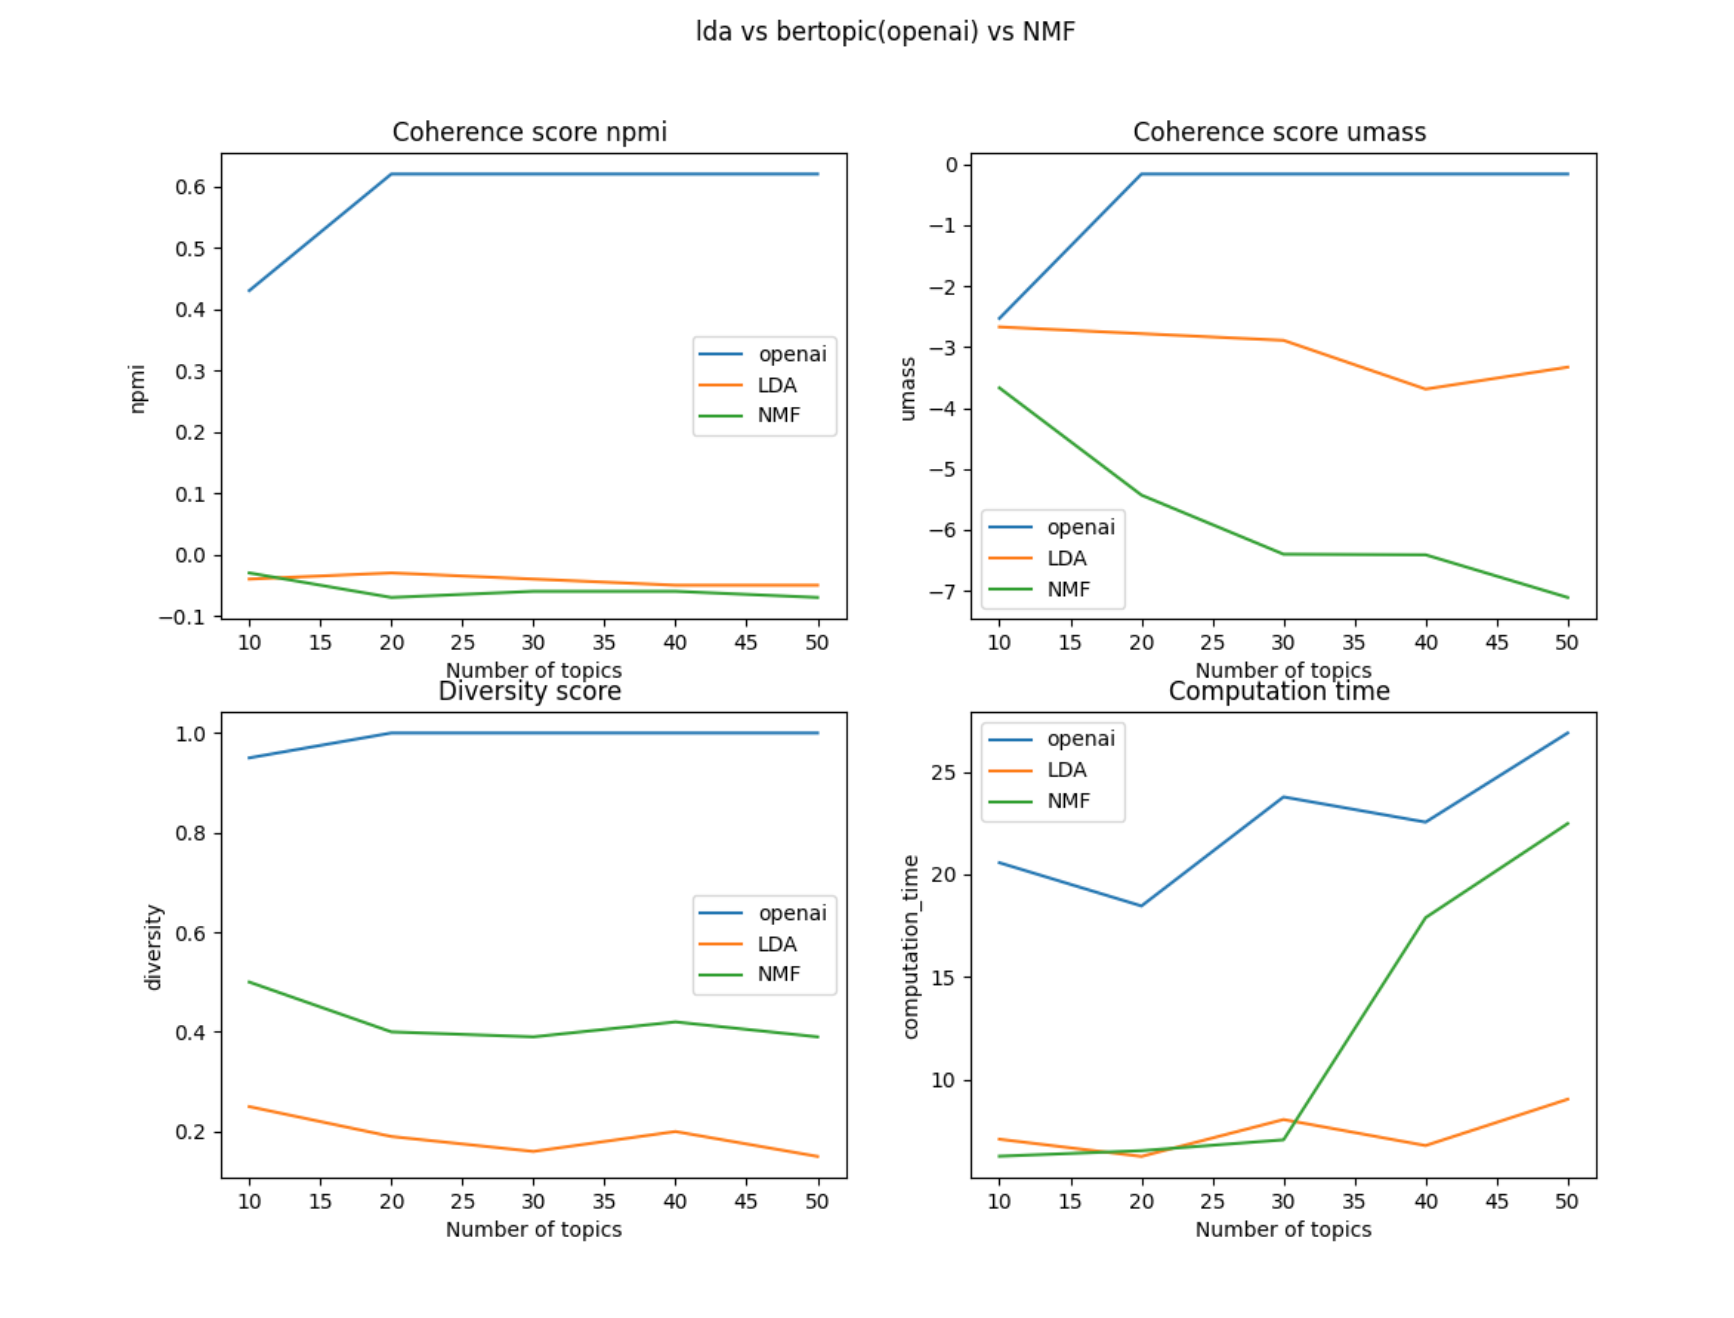
\includegraphics[width=0.99\linewidth]{Chapter4/figures/topic_unsupervised.png} 
    \caption{coherence and diversity for LDA, BERTopic, and NMF
    }
    \label{figure:unsupervised_results} % assign a unique label to each figure
\end{figure}


However, Hoyle et al  \cite{hoyle_is_2021} showed how these metrics are not very meaningful for evaluating these models and we should take these results with a grain of salt.

From this evaluation, we can conclude that for BERTopic the topic size is better bigger than smaller especially if we have many documents. Topics of Bertopic are way more diverse than LDA and NMF and within the topics, the most relevant word are more semantically related.


\subsection{Supervised}
Considering the result of the unsupervised evaluation we should use another method to validate what we found. In this case, we created two ad hoc datasets to see too how the models perform in a real-case scenario.

\paragraph{Dataset}

The first step for the supervised part was the data collection, in this case, we packed specific datasets to test our models. The first is simpler and contains very different topics so that should be easy to cluster the documents, while the second is more trickier because it contains only politics-related tweets with some overlapping.

\begin{itemize}
    \item \textbf{simple}: 1093 labeled tweets of 5 different topics identified by a hashtag \footnote{\#Bitcoin, \#stormydaniels, \#UkraineRussianWar, \#SaudiArabianGP, \#climatechange}
    \item \textbf{politics}: 1492 labeled tweets of 7 politics-related hashtags \footnote{\#IndictArrestAndConvictTrump, \#kabul, \#BidenHarris2024, \#KamalaHarris, \#taiwan, \#belarus,  \# stormydaniels}
\end{itemize}


For both datasets, we used two different versions: with and without hashtags.

The tweets have been extracted using \href{https://twarc-project.readthedocs.io/en/latest/twarc2_en_us/}{twarc2} getting only English tweets and without retweets.

\paragraph{Metrics}
In order to evaluate the topics we had to define some metrics:

\begin{itemize}
    \item \textbf{Accuracy}: for each known topic look at the biggest of inferred topics and divide by the number of tweets in that topic.
    \item \textbf{Accuracy no outliers}: in the Bertopic case the label -1 refers to outliers.
    \item \textbf{Min\_topic\_share}:  same as accuracy but in the opposite direction, after having computed it for all of my\_topics we take the minimum
\end{itemize}


\paragraph{Parameters}

\begin{verbatim}
BERTopic: (nr_topics = 'auto', min_topic_size = 50)

NMF: (max_df = 0.95, min_df = 3, ngram_range = (1,2))

GSDMM: (alpha = 0.1, min_df = 0.1, n_iters = 30)
\end{verbatim}


\paragraph{Simple Dataset Results}
We started evaluating the \textit{simple} dataset with hashtags and as we can see in Fig \ref{figure:supervised bar} base ( all-MiniLM-L6-v2) and OpenAi obtained almost a perfect score for each topic, while climatebert seems to have a great accuracy but a low mean topic share, this is a signal that something is wrong and we should inspect the heatmap.

\begin{figure}[h]
    \centering % figure is centered on the page
        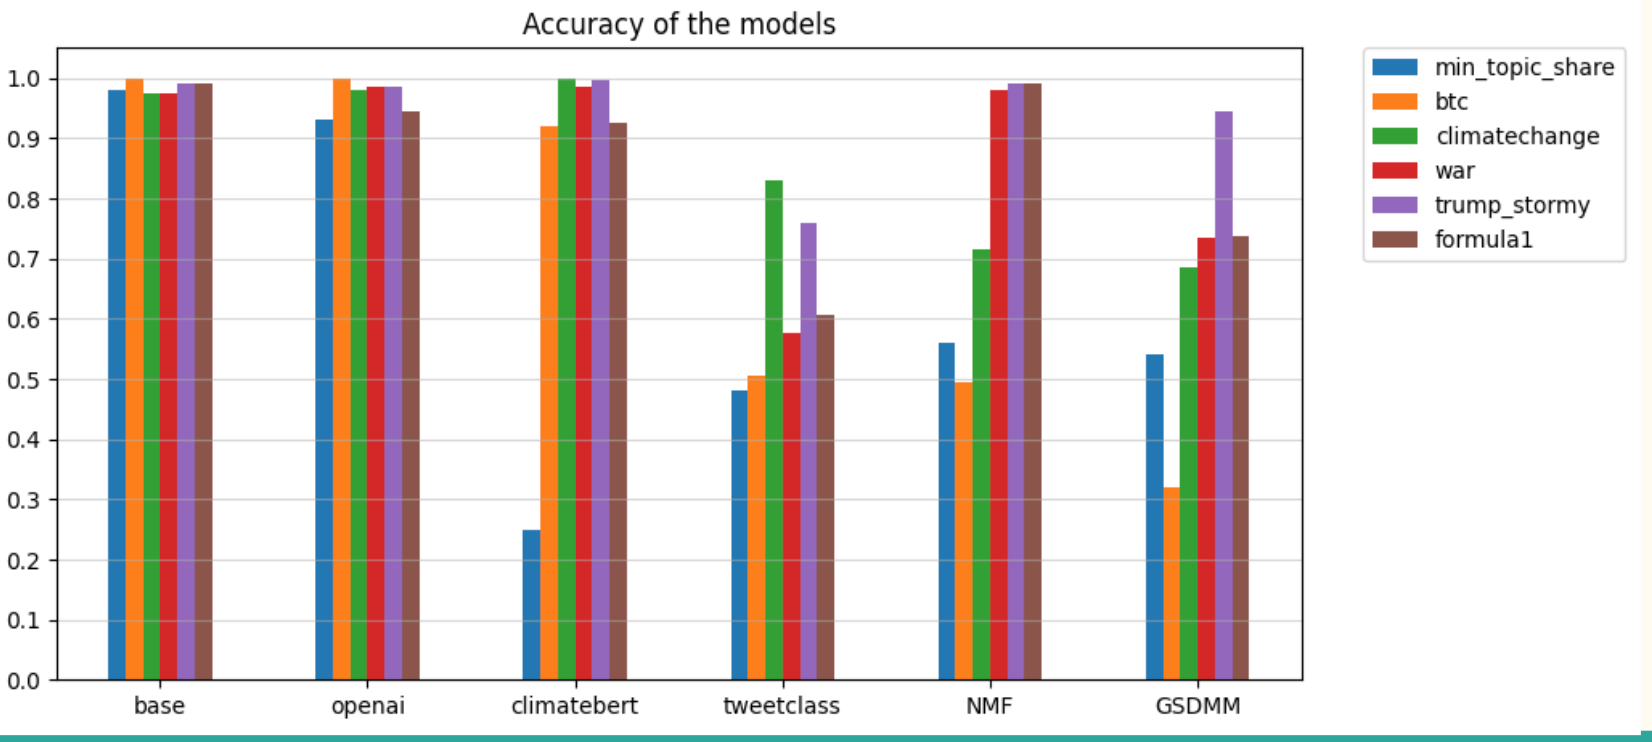
\includegraphics[width=0.99\linewidth]{Chapter4/figures/topic_supervised_bar.png} 
    \caption{All models accuracy simple  with hashtags
    }
    \label{figure:supervised bar} % assign a unique label to each figure
\end{figure}

In fact, we can clearly see in \ref{figure:sup_heatmap1_simple_hash} that even though the accuracy is very good, climatebert has some difficulties in dividing the topics putting almost all the tweets in the same. While the first two are performing very well as expected it is not true for the others. We can see how climate bert put almost all the tweets in topic 0, being able only to find the formula1 tweets and not the climatechange one, as it is designed to do.
That’s the reason why we decided to remove the models that are not performing well in the simplest case with the exception of NMF to use it as ground truth. 


\begin{figure}[h]
    \centering % figure is centered on the page
        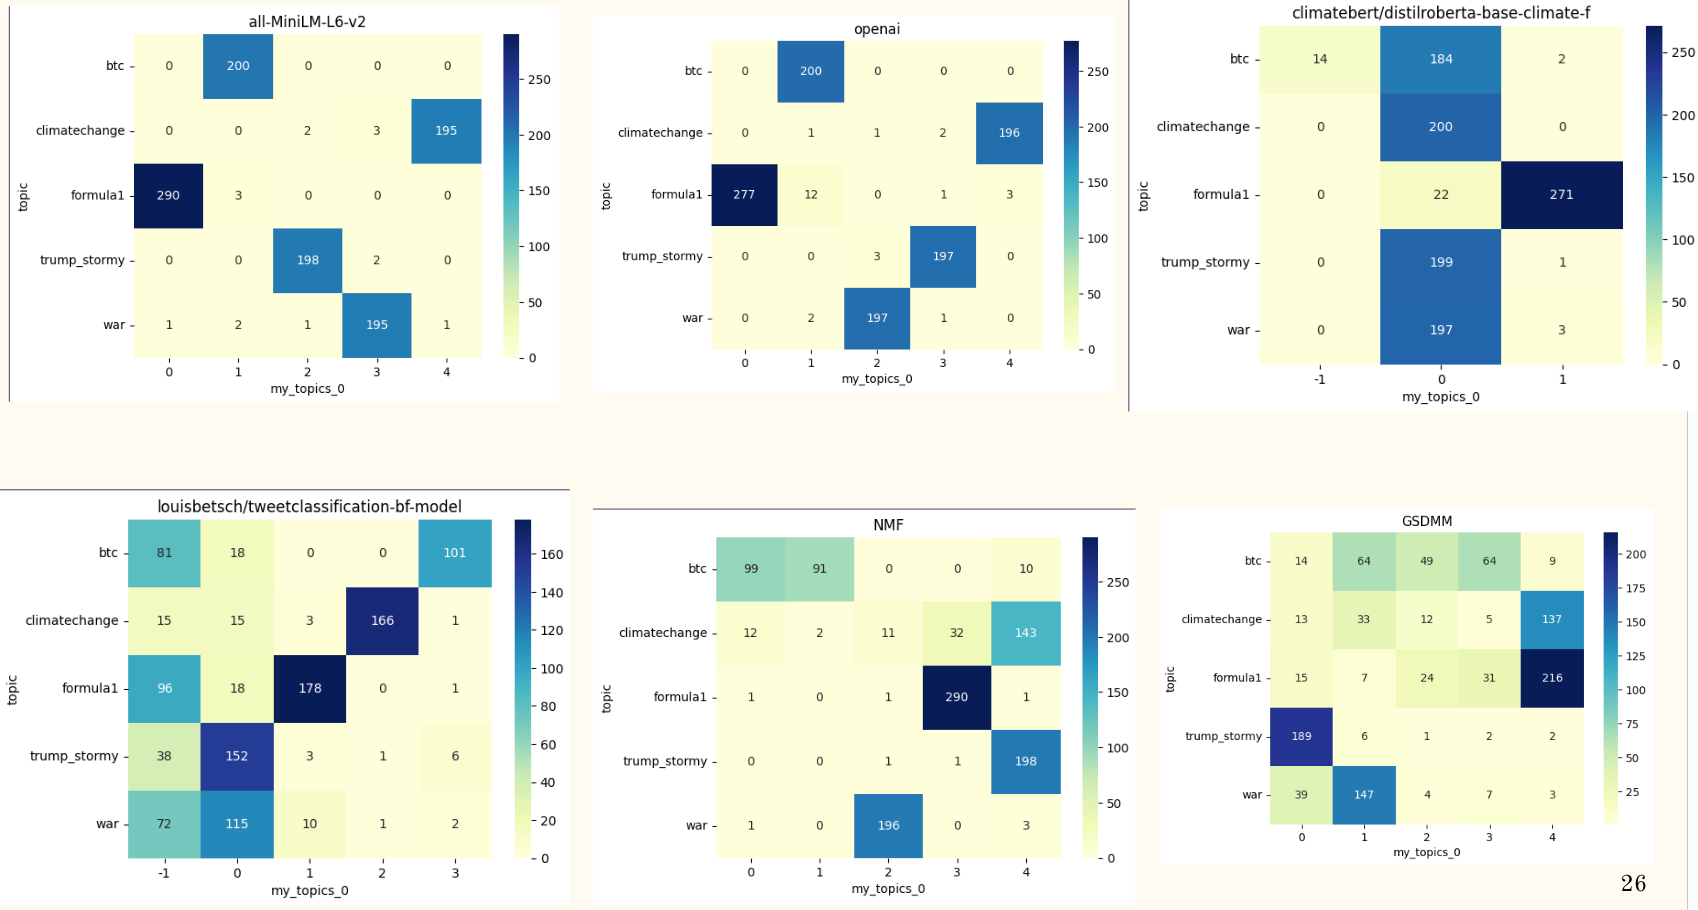
\includegraphics[width=0.99\linewidth]{Chapter4/figures/topic_heatmap1.png} 
    \caption{Heatmap comparison of the different model with the simple dataset with hashtags
    }
    \label{figure:sup_heatmap1_simple_hash} % assign a unique label to each figure
\end{figure}

Looking at \ref{figure:supervised heatmap1} we can see how BERT and OpenAI performed in the same dataset but without the hashtags, in particular how BERT tends to find more outliers than OpenAI.


\begin{figure}[h]
    \centering % figure is centered on the page
        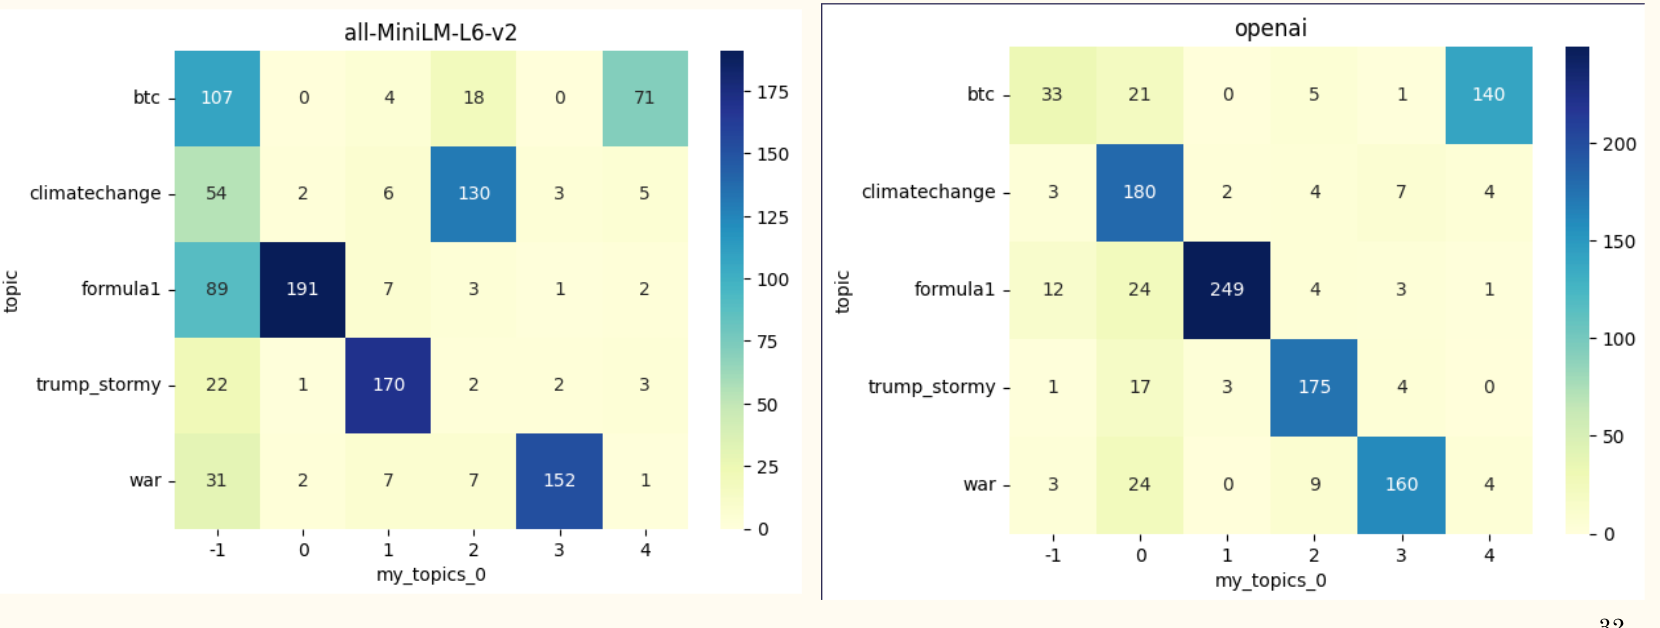
\includegraphics[width=0.99\linewidth]{Chapter4/figures/topic_heatmap_bertopic.png} 
    \caption{Heatmap comparison of mini and OpenAi of the simple dataset without hashtags}
    \label{figure:supervised heatmap1} % assign a unique label to each figure
\end{figure}
An interesting feature of Bertopic is the ability to visualize the different topics in a 2-dimensional space, Fig \ref{fig:openai docs} show the document distribution of OpenAi after projecting the embeddings in a two-dimensional space.
\begin{figure}
    \centering
    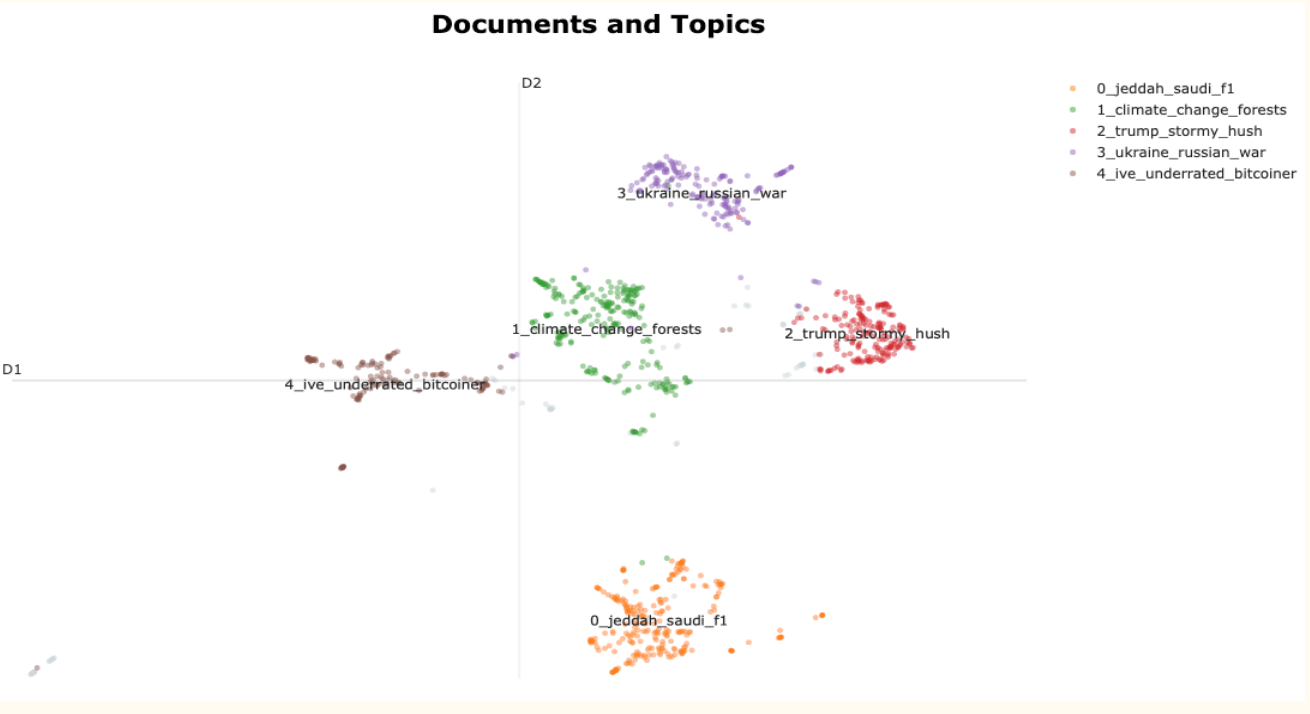
\includegraphics[width=1\linewidth]{Chapter4/figures/openai_documents_viz.png}
    \caption{docs representation of simple dataset for openai}
    \label{fig:openai docs}
\end{figure}


\paragraph{Politics dataset results}

The politics dataset is clearly more difficult to evaluate but with the hashtags it is still doing a good job. Even though we can see that both BERT and OpenAi are merging two topics. In particular, for OpenAi makes more sense since the two hashtags related to Trump are related to the same event( \#trump and \#trump\_stormy

\begin{figure}
    \centering
    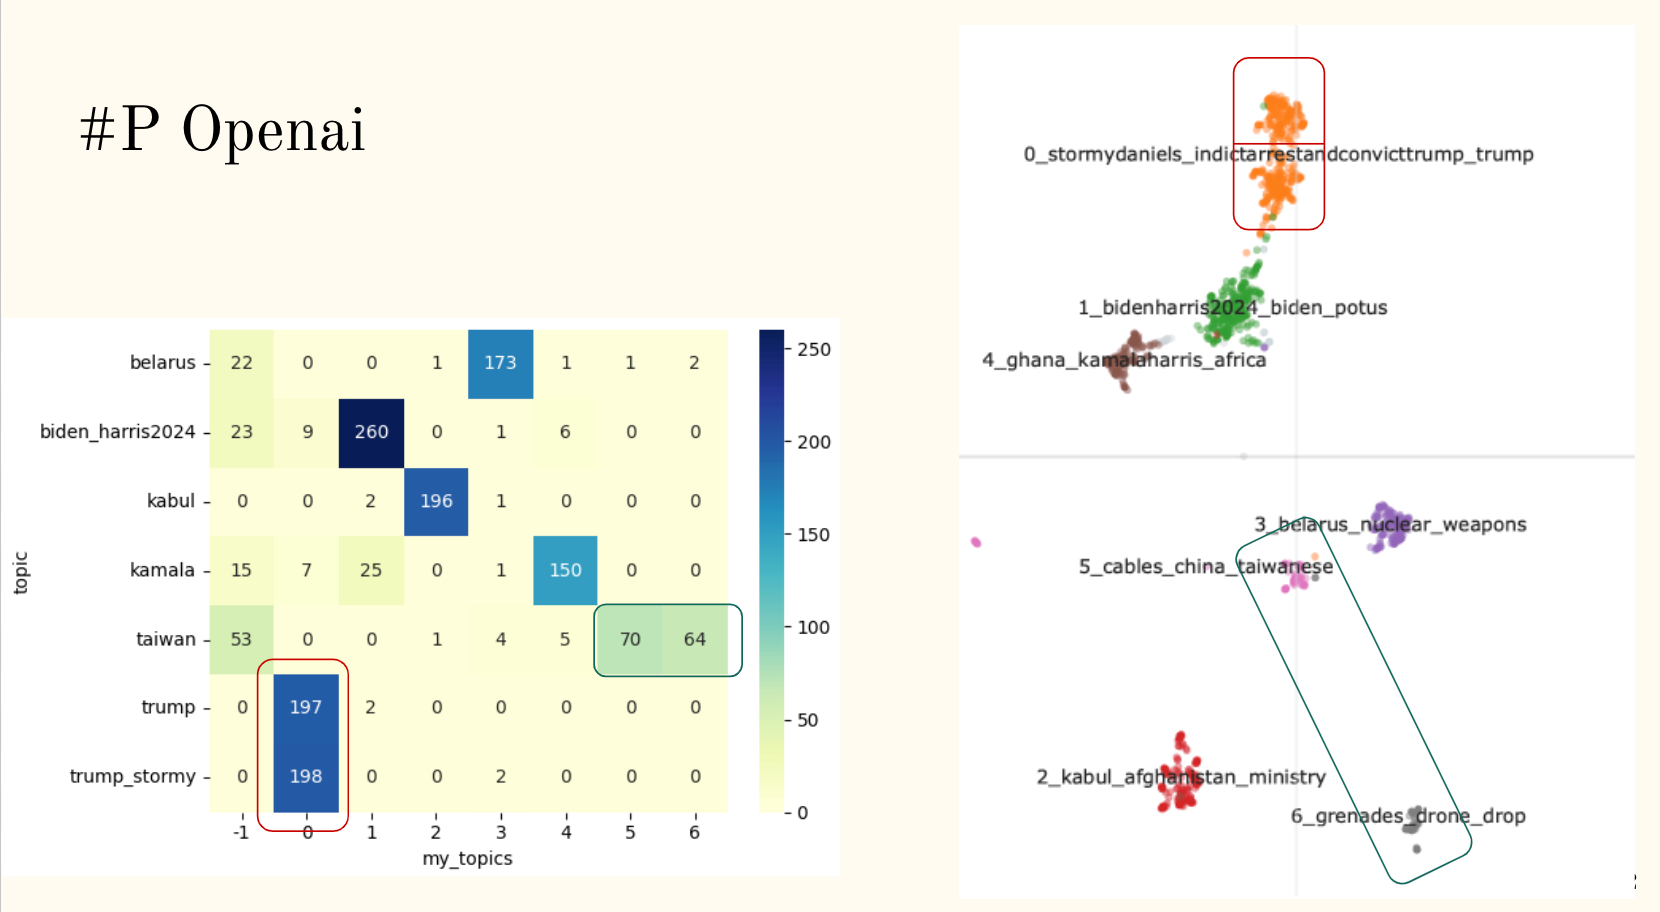
\includegraphics[width=1\linewidth]{Chapter4/figures/openai_politics_hash_comparison.png}
    \caption{Heatmap and documents representation of the politics dataset with hashtags evaluated with openai}
    \label{fig:openai_heat_docs_politics_hash}
\end{figure}

To validate the results we run the algorithm 100 times and most of the time for BERT the min topic share is 0.9 which means they got the correct number of topics and classified them in a good way. We can look at Fig \ref{fig:bert politics with hashtags} to see both documents and the heatmap.

\begin{figure}
    \centering
    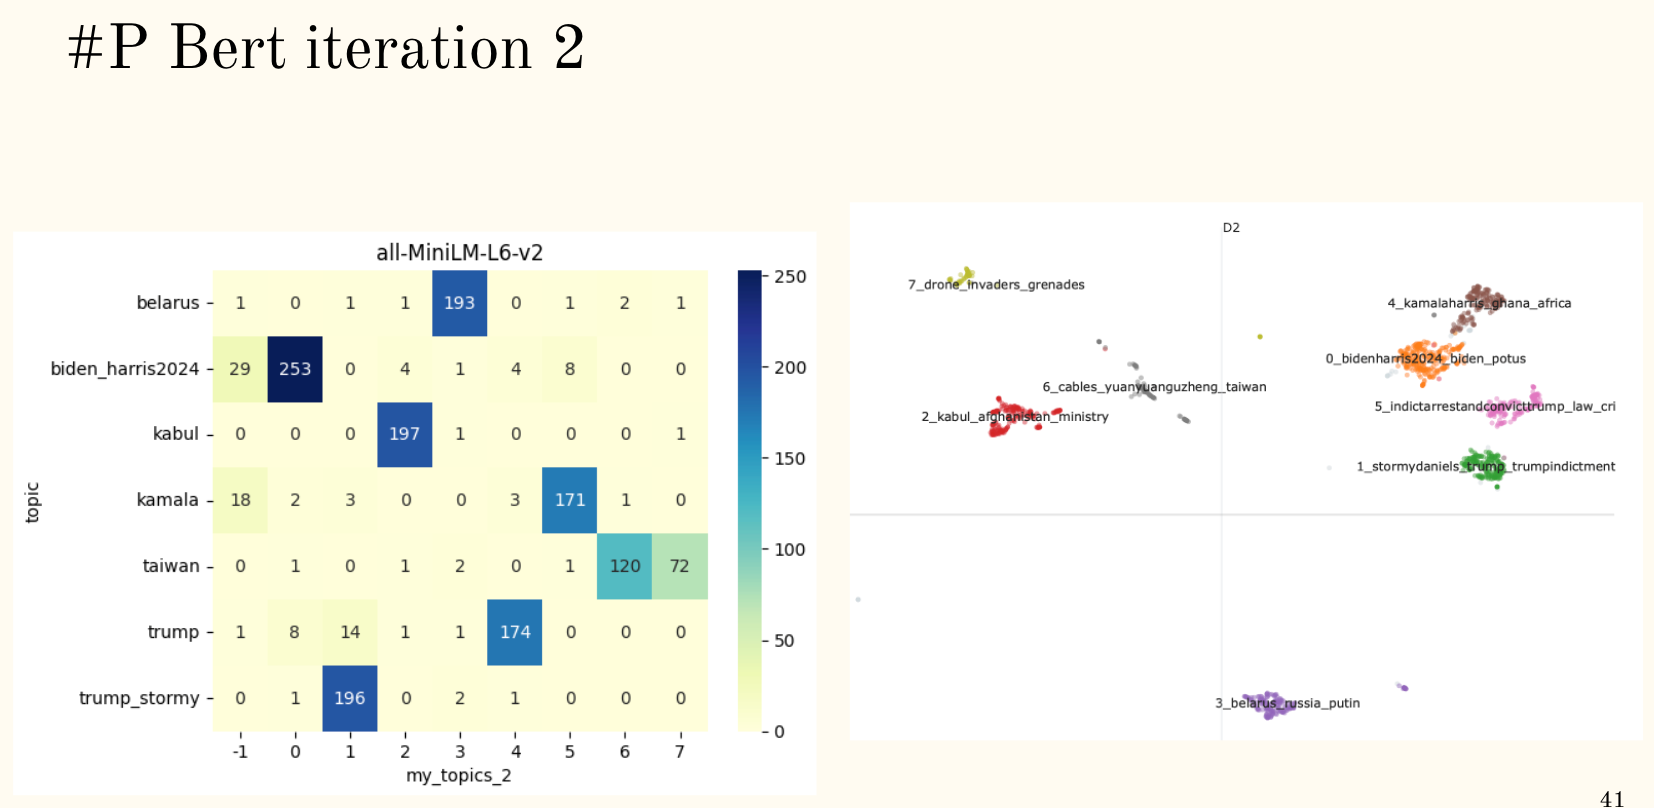
\includegraphics[width=1\linewidth]{Chapter4/figures/bert_politics_hash_comparison.png}
    \caption{bert heatmap and document viz politics with hashtags}
    \label{fig:bert politics with hashtags}
\end{figure}
in the case without hashtags OpenAi and BERT put in a single cluster all the tweets related to American politics both also understanding that Kamala's tweets were about something else.

\paragraph{Conclusion}
Tab \ref{tab:unsupervised_recap} show the result of unsupervised evaluation, while Tab \ref{tab:supervised recap } the supervised


\begin{table}[]
\centering
\begin{tabular}{|llll|}
\hline
\textbf{model}                              & \textbf{npmi} & \textbf{umass} & \textbf{diversity} \\ \hline
\multicolumn{1}{|l|}{tweet\_classification} & 0.62          & -0.16          & 1                  \\
\multicolumn{1}{|l|}{openai}                & 0.58          & -0.63          & 0.99               \\
\multicolumn{1}{|l|}{climatebert}           & 0.20          & -2.28          & 0.83               \\
\multicolumn{1}{|l|}{U.S.E}                 & 0.20          & -4.35          & 0.89               \\
\multicolumn{1}{|l|}{BERT}                  & 0.20          & -5.46          & 0.97               \\
\multicolumn{1}{|l|}{LDA}                   & -0.04         & -3.07          & 0.19               \\
\multicolumn{1}{|l|}{NMF}                   & -0.06         & -5.80          & 0.42               \\ \hline
\end{tabular}
\caption{all the models tested in the unsupervised evaluation}
\label{tab:unsupervised_recap}
\end{table}

\begin{table}[]
\centering
\begin{tabular}{|l|ll|}
\hline
model  & accuracy & topic share \\ \hline
BERT   & 0.84     & 0.86        \\
OpenAI & 0.83     & 0.85        \\
NMF    & 0.78     & 0.69        \\ \hline
\end{tabular}
\caption{recap of supervised evaluation}
\label{tab:supervised recap }
\end{table}



\section[Networks]{Networks}

A network, often referred to as a graph, is a data structure that is composed of nodes and ties, which represent the connections between the nodes. This interconnected structure allows for the representation and analysis of relationships and dependencies among various entities. The applications of networks are incredibly diverse and wide-ranging.

One example of a network is a computer network, which consists of interconnected computers that communicate and share resources. Another example is a network of webpages, where each webpage is represented as a node, and the links between webpages form the ties. This type of network is fundamental to the World Wide Web and enables the navigation and discovery of information online. Additionally, networks find applications in logistics and transportation, where they are utilized to optimize routes and streamline the movement of goods and service. These are only few examples in the use of networks, in this thesis the focus will be on social networks, where the nodes represents persons and the tie some sort of interaction between them.


Social Network Analysis is a field that examines the relationships, the interactions, and the structures within a network of individuals or entities. It provides valuable insights into the dynamics, information flow, and influence within social networks. Several studies have
 applied SNA in different domains \cite{borgatti_network_2009}, such as online social networks, organizational networks, and public health networks. A growing field in this context is the analysis of social media, which completely changed how the research in this area is carried out. Due to the huge amount of data available, it is possible to shift to a data driven methodology, where the data collection is not strictly embedded in the design of the experiment, but it is the starting point on top of which the research is built. Another advantage of this kind of data is that, since it results from a natural observation of actors in a social environment, it is not as biased as self-reported data or as data collected in a laboratory setting. Concerning this, Veltri \cite{digital_veltri_2019} explains how behavioral data is linked to automatic decisions in the surrounding environments, while the self reported one is more conscious and reflexive and not always the action matches what people say. It must be noted that the data is not completely unbiased, it depends on the goal and the structure that the platform gave to it.

In this scenario, the data is being used to explore the topology of the interaction between users of Twitter; the structure of their interactions is studied to understand if there are some recurring patterns.

\subsection{Multi-layer Networks}
In particular, we will build our network using a Multi-layer networks (MLN) framework\cite{kivela_multilayer_2014}. MLN are complex networks that capture multiple types of relationships, or interactions, between nodes. They allow for the representation of different dimensions or contexts in a single framework, providing a more comprehensive understanding of network dynamics. Single-layer networks are, in certain cases, an oversimplification of reality\cite{trax_multilayer_16} \cite{hammoud_multilayer_2020}.

MLN are often used in biological networks where, due to organism complexity, every biological function is usually influenced by more factors, and modeling with a MLN helps the researcher in studying the interaction between these factors. Another biological use of MLN is epidemiology, where the presence of a certain disease can be strongly influenced by other clinical conditions. For example Kinsley et al. \cite{kinsley_multilayer_2020} used this framework in veterinary epidemiology to identify the subjects that are more prone to spread a certain disease.

Also in the field of interest for this research, social networks and, in particular, Twitter, several researchers used MLN to structure their study: for instance ref \cite{nguyen_twitter_21} employed it to identify the most central accounts over multiple layers in the discussion of different political candidates, one for each layer. In relation to this, De Domenico \cite{de_domenico_ranking_2015} mathematically described different ways to compute node centrality on multiple layers, introducing the concept of versatility.

Thanks to the complexity added by the multiple layers, the same users can be seen interacting in the different dimensions, which in our case are the different topics. This implies that for each identified topic In the topic modeling phase, it is possible to observe a network of interactions among users, allowing the study of the users’ presence on multiple topics.




\section[Polarization]{Polarization}
As anticipated in chapter \ref{Introduction}, it is fundamental for the understanding of this work to comprehend what Falkenberg did in his research \cite{falkenberg_growing_2022}. Since the same methods are employed here, we also make the same assumption of the bipolarity of the polarization. In this section, it will be shown  how polarization will be computed.

A meaningful metric that gained popularity among social scientists is polarization. The researchers believe that polarization can be harmful for the maintenance of the democratic stability \cite{mccoy_polarization_democracy_2018}. Thus, understanding the phenomenon is important to develop a solution to it.

Polarization has been used to study the impact of political discussion on social media, especially around US presidential elections  \cite{conover_political_2011}
\cite{flamino_shifting_2021} . Due to this, attention should be paid when generalizing, especially since US politics are built around two main parties -Democrats and Republicans-, making a bimodal view of polarization the best suited for this case (but not for all). Despite this, an analysis of the polarization over 21 different countries shows that the US is not the only place where it has been detected  \cite{gidron_toward_2019}. Ref
\cite{radicioni_networked_2021}
show the polarization can have different geometries than the traditional bimodality.

Even though Falkenberg detected an increasing polarization only in the COP26, while in 2015, Williams et al. \cite{williams_network_2015} found the presence of echo chambers around the climate discussion in social media, with a small presence of open forums. In this work, there will be an attempt to connect these two pieces of research, to understand if, by breaking down the discussion into topics, the polarization of specific topics has always been high.

There is not a clear and universally adopted definition of polarization; Bramson et al. \cite{bramson_understanding_2017} tried to summarize it by defining different types of it; the assumption is that there is a measure of ’opinion’ for each user: 
\begin{itemize}
    \item \textbf{Spread} defines the distance between the two extremes as the breadth of opinion
    \item \textbf{Dispersion} considers the shape of the distribution of the opinions and searches for peaks
    \item \textbf{Coverage} does not look at the shape but at the similarity of opinions within the groups
    \item \textbf{Regionalization} looks at the spectrum not covered between the groups
    \item \textbf{Community fractioning} is the degree to which the population can be broken into subpopulations
    \item \textbf{Distinctness} is defined as  "the degree to which the group distribution can be separated"
    \item \textbf{Group divergence} is the opposite of distinctness, how different are the groups
    \item  \textbf{Group consensus} shoes how people in the same group have similar opinions
    \item  \textbf{Size parity } put relevance on the size of each group
\end{itemize}



We use the definition of Dispersion polarization that looks into the distribution of beliefs to detect peaks. Falkenberg demonstrated that the assumption of bimodality makes sense when dividing the population into climate supporters and climate skeptics. There is also the assumption  that  the polarization can be detected using the retweet network.

\paragraph{Latent ideology}
In order to compute polarization on a retweet network, firstly,  a latent ideology for each user is to be estimated, as defined in \cite{barbera_birds_2015} and adapted for retweets in \cite{flamino_shifting_2021}.


Starting from the adjacency matrix of the retweet network, and after some linear algebra, a latent ideology score for each user can be obtained.

The first step is to identify \textit{m }most retweeted users -from now on \textit{influencers- }, out of the \textit{n }users, and then build an adjacency matrix $A\in \mathbb{R}^{n x m}$ between users and influencers (where \(a_{ij}\) is the number of times user $i$ retweeted influencer $j$).  Now the process will be shown in detail from the matrix to the scores. In this way all the users that did not interact with the top $m$ influencers will be excluded from the analysis.

\\

Firstly, normalize $A$ by the number of retweets:
\begin{equation}
P =  \frac{A_{ij}}{\sum_{i} \sum_{j} a_{ij}}
\end{equation}

Secondly, get the vector of row and column sums and consider the diagonal matrix:
\begin{equation}
\textbf{r} \in \mathbb{R}^m, \quad  r_i = \sum_{i} a_{ij}
\end{equation}
\begin{equation}
\textbf{c} \in \mathbb{R}^n , \quad c_j = \sum_{j} a_{ij} 
\end{equation}





\begin{equation}
  R =
  \begin{bmatrix}
    \frac{1}{{\sqrt{r_{1}}}} & & \\
    & \ddots & \\
    & & \frac{1}{{\sqrt{r_{n}}}}
  \end{bmatrix}
  \;\;\;  C =
  \begin{bmatrix}
    \frac{1}{{\sqrt{c_{1}}}} & & \\
    & \ddots & \\
    & & \frac{1}{{\sqrt{c_{n}}}}
  \end{bmatrix}
\end{equation}

Then, compute the matrix of standardized residuals $S$:
\begin{equation}
S = R\left(P - (\textbf{r}\cdot \textbf{c}^T)\right)C
\end{equation}

Using Singular Value Decomposition (SVD), which is a factorization technique in linear algebra,  the standardized matrix  can be decomposed into three other matrices. It provides essential geometrical and theoretical insights about linear transformations and it is extensively used in various fields such as data science, engineering, and statistics \cite{golub1970singular}. Given  matrix $S$, its SVD is  written as:

\begin{equation}
S = U\Sigma V^T
\end{equation}

where $U$ is an $m \times m$ matrix whose columns are the orthonormal eigenvectors of $AA^T$, $\Sigma$ is an $m \times n$ diagonal matrix whose non-zero elements are the singular values of $A$, and $V^T$ is the transpose of an $n \times n$ matrix whose columns are the orthonormal eigenvectors of $A^T A$. The singular values on the diagonal of $\Sigma$ are typically sorted in descending order. The columns of $U$ and $V$ are called the left-singular vectors and right-singular vectors of $A$, respectively.
\\

Multiply $R$ and $U$:
\begin{equation}
X = R U
\end{equation}

Finally, rescale $U$ on $[-1,1]$ and get the user score:
\begin{equation}
score = -1 + 2 \cdot \frac{{X} - \min(X)}{\max(X) - \min(X)}
\end{equation}








\paragraph{Hartigan's diptest}

After computing all the users' latent ideology scores, to test the polarization,   Hartigan's diptest is used \cite{hartigan_dip_1985}.

Hartigan's Dip Test is a statistical test used to determine if a distribution is unimodal. The test works by comparing the empirical distribution function of the data, denoted as $F(x)$, to the unimodal distribution function that minimizes the maximum difference between $F(x)$ and itself, denoted as $G(x)$. The dip statistic $D$ is then defined as:

\begin{equation}
D = \sup_x |F(x) - G(x)|
\end{equation}

Where $\sup_x$ denotes the supremum (least upper bound) overall $x$, the unimodal distribution function $G(x)$ is chosen so that it minimizes this supremum. In other words, $G(x)$ is the "best" unimodal approximation to the empirical distribution function $F(x)$.

The null hypothesis of the Dip Test is that the data comes from an unimodal distribution. If the dip statistic $D$ is significantly large, the null hypothesis  is rejected and the conclusion is that the data is not unimodal. The p-value of the test is computed by comparing the observed dip statistic to the distribution of the dip statistic under the null hypothesis. This distribution is typically approximated using Monte Carlo simulations.






%!TEX root = ../thesis.tex
%*******************************************************************************
%****************************** Third Chapter **********************************
%*******************************************************************************
\chapter{Data Description}%Make this title more interesting
In this chapter we will see an overview of the starting data used in this research, as well as some general statistics about it.

\section{Where the data comes from}
The data are tweets collected from the twitter api containing the hashtag \#cop21 #cop26. 
For each cop we have two jsonlines files, one for the tweets and one for the users involved. The fields are the one stated in the documentation \footnote{ \href{https://developer.twitter.com/en/docs/twitter-api/data-dictionary/object-model/tweet}{https://developer.twitter.com/en/docs/twitter-api/data-dictionary/object-model/tweet}}, there are many fields but the relevant ones are the following: 

\begin{table}[H]
\centering
\begin{tabular}{|l|l|}
\hline
\textbf{Field} & \textbf{Description} \\ \hline
author & The ID of the author \\ \hline
author\_name & The username of the author \\ \hline
text & The text of the tweet \\ \hline
date & The creation date of the tweet \\ \hline
lang & The language of the tweet \\ \hline
conversation\_id & The ID of the conversation the tweet belongs to \\ \hline
referenced\_type & The type of the referenced tweet \\ \hline
referenced\_id & The ID of the referenced tweet \\ \hline
mentions\_name & The usernames of the mentioned users in the tweet \\ \hline
mentions\_id & The IDs of the mentioned users in the tweet \\ \hline

\end{tabular}
\caption{Description of the fields used of the tweets data}
\label{tab:my_label}
\end{table}
While we use the user's file to map the id of the users to their username, even though not always we have this information, in that case we use the user id as username

\section{Some statistics}
We have data from 2 cops: COP21 , COP26.
we call original tweet a tweet that has been written by an user, so that's not a retweet. Fig \ref{fig:tweets_by_date} show the tweets distribution over the time for both cops, most of the tweets have been tweet during while the conferences were taking place.

\begin{figure}[H]
    \centering
    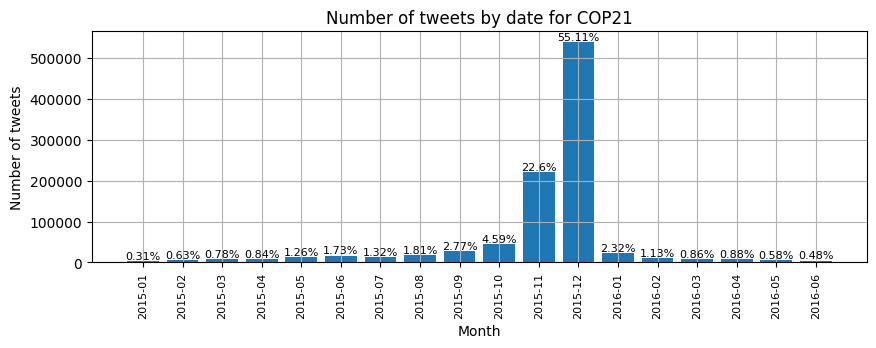
\includegraphics[width=0.75\linewidth ]{Chapter3/figures/tweets_by_date_cop21.png}

    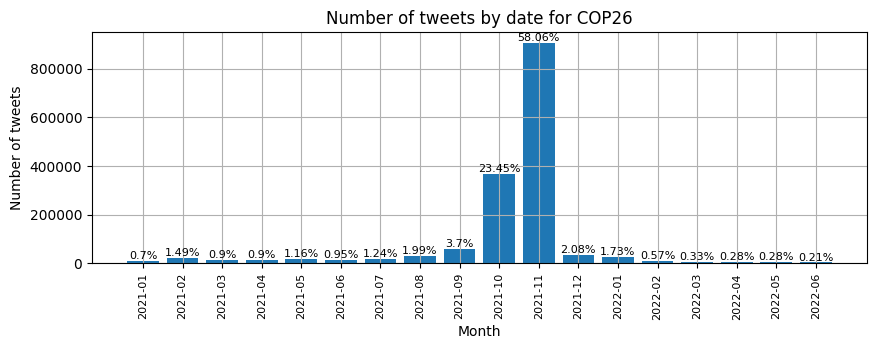
\includegraphics[width=0.75\linewidth ]{Chapter3/figures/tweets_by_date_cop26.png}
    \caption{Numebr of tweets by date for cop 21 and cop26}
    \label{fig:tweets_by_date}
\end{figure}

\paragraph{COP21}
The date of the tweets spans from january 2015 to june 2016 but 77\% of the tweets are from november and december 2021, cop26 has been held between 30th novemebr and 12th december. In the dataset there are 975040 tweets that have been tweeted by 234389 users of which only tofix tweeted an original tweets with at least one retweet, every users tweeted on average 4.16 tweets, the maximum amount of tweet a user tweeted is 9635, 89\% of users tweeted less than 5 tweets.

\paragraph{COP26}
The date of the tweets spans from january 2021 to july 2022 but 81\% of the tweets are from October and November 2021, cop26 has been held between 31th october and 12th november. In the dataset there are 1558968 tweets that have been tweeted by 456000 users of which only 30195 tweeted an original tweets with at least one retweet, every users tweeted on average 3.42 tweets, the maximum amount of tweet a user tweeted is 14267, 90\% of users tweeted less than 2 tweets.
\\


Fig \ref{fig:tweets_by_users} shows how most of the users tweeted just few tweets (note that it is logarithmic) in the case of cop26 there \% of users tweeted less than 5 tweets, for cop21.

\begin{figure}
    \centering
    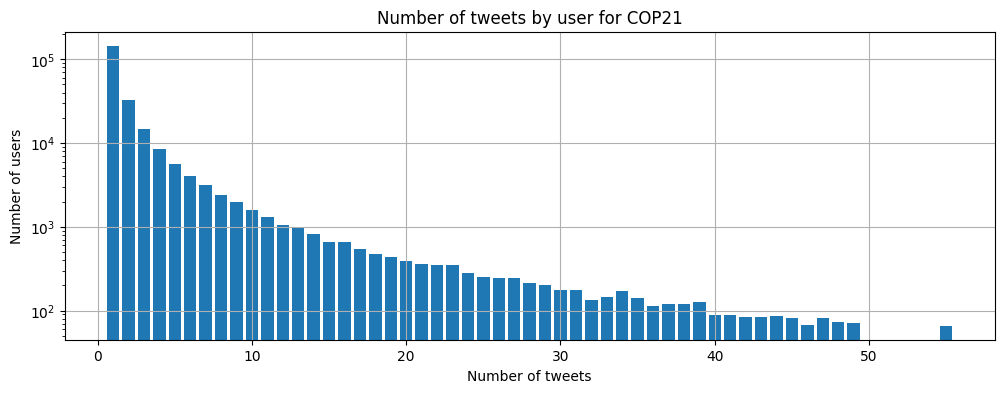
\includegraphics[width=0.75\linewidth ]{Chapter3/figures/tweets_by_users_cop21.png}

    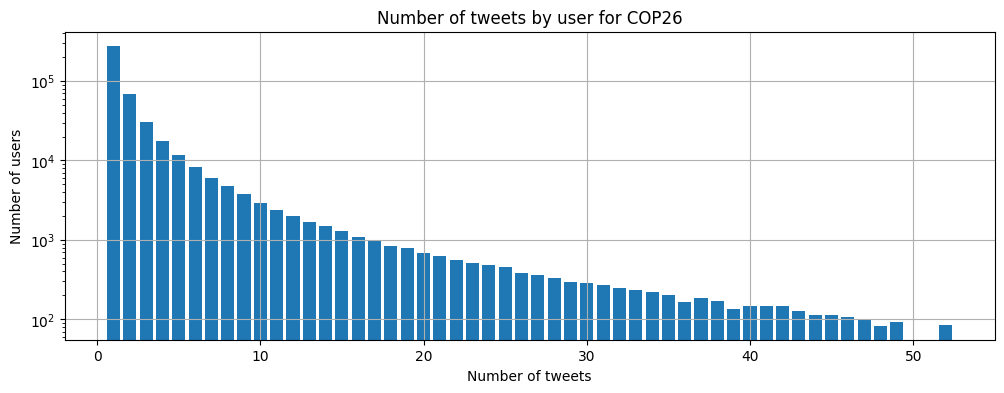
\includegraphics[width=0.75\linewidth ]{Chapter3/figures/tweets_by_users_cop26.png}
    \caption{Numebr of tweets by user for cop 21 and cop26}
    \label{fig:tweets_by_users}
\end{figure}






\begin{table}[h]
\centering
\setlength{\tabcolsep}{10pt} % Sets the horizontal padding
\renewcommand{\arraystretch}{1.5} % Sets the vertical padding
\begin{tabular}{
  |l|
  S[table-format=7.0,group-four-digits=true]|
  S[table-format=7.0,group-four-digits=true]|
  S[table-format=7.0,group-four-digits=true]|
  S[table-format=7.0,group-four-digits=true]|
}
\hline
 & {\textbf{n\_tweets}} & {\textbf{n\_retweets}} & {\textbf{n\_original}} & {\textbf{n\_original\_with\_retweets}} \\ \hline
\textbf{COP21} & 975040 & 562946 & 412094 & 138427 \\ \hline
\textbf{COP26} & 1558968 & 1191813 & 367155 & 130138 \\ \hline
\end{tabular}
\caption{Number of tweets}
\label{tab:n_tweets}
\end{table}




in fig \ref{fig:cop26_tweets_stats} we can see how the 1'558'968 are distributed, in fact 76\% of them are retweets generated by only 130k original tweets. It is also worth nothing that almost 2/3 of the original tweets have 0 retweets 

\begin{figure}
    \centering
    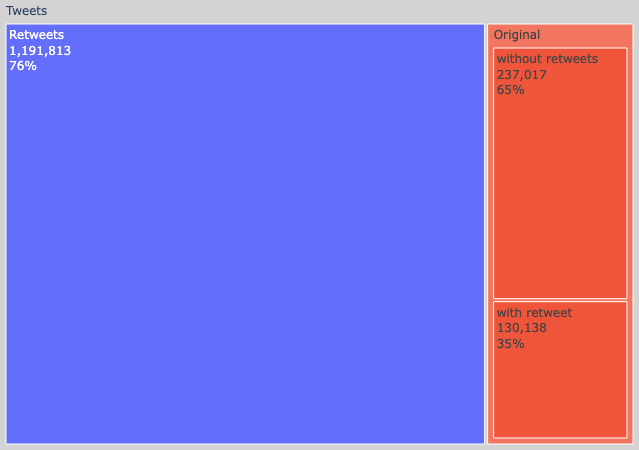
\includegraphics[width=0.9\linewidth]{Chapter3/figures/treemap_tweets-1.png}
    \caption{tweets of cop26}
    \label{fig:cop26_tweets_stats}
\end{figure}








% **************************** Define Graphics Path **************************
\ifpdf
    \graphicspath{{Chapter3/Figs/Raster/}{Chapter3/Figs/PDF/}{Chapter3/Figs/}}
\else
    \graphicspath{{Chapter3/Figs/Vector/}{Chapter3/Figs/}}
\fi


\chapter{Methodology}
In this chapter we will 

\section{Topic Modeling Evaluation}

    \graphicspath{{Chapter4/Figures}{Chapter4/Figures}}

In this chapter, the evaluation of different models used for tweet labeling is presented. Both unsupervised and supervised approaches were used to evaluate the performance of the models. 
The goal of the evaluation was to find the best-performing model to accurately label tweets. 
The models used included traditional methods (LDA, GSDMM, and NMF) as well as neural models like  BERTopic. Evaluation metrics such as coherence and diversity were used to compare the different models. The results showed that BERTopic performed better than traditional methods, especially when using all-MiniLM-L6-v2 (BERT) \footnote{\href{https://huggingface.co/sentence-transformers/all-MiniLM-L6-v2}{huggingface.co/sentence-transformers/all-MiniLM-L6-v2}}
, text-embedding-ada-002 (OpenAI) \footnote{\href{https://platform.openai.com/docs/models/embeddings}{platform.openai.com/docs/models/embeddings}}, and tweet\_classification \footnote{\href{https://huggingface.co/louisbetsch/tweetclassification-bf-model}{huggingface.co/louisbetsch/tweetclassification-bf-model}} embeddings. The supervised evaluation showed that BERT and OpenAI were the best-performing models. The section concludes with a summary of the results and a description of the representation used for labeling the tweets.

The models used are both traditional(LDA, GSDMM, NMF) as a reference of the ground truth and neural because seem to be the most accurate, in particular, we will evaluate BERTopic with several embedding methods. We choose BERtopic over Top2Vec because they are very similar and also because the Python library is more complete and allows us to be more flexible.

Evaluating a topic modeling algorithm is not a straightforward task due to the lack of objectivity in identifying a topic. In this work we evaluated the models in two ways: first using a widely used unsupervised approach: metrics like coherence and diversity. 
Then to validate the results we also did a supervised evaluation using different datasets built ad hoc for this setting.

\subsection{Unsupervised}
To compare the different models we used a library suggested by the creator of BERtopic called OCTIS \cite{DBLP:conf/clic-it/TerragniF21} \cite{terragni2020octis}, this allowed us to structure an experiment to measure different metrics:

\paragraph{Metrics}

\begin{itemize}
    \item \textbf{NPMI coherence:} degree of association between the top words in a topic
    \item \textbf{Umass coherence}: how often two words appear together
    \item \textbf{Diversity}: how distinct the topics are from each other
    \item \textbf{Computation time}: time needed to fit the models
\end{itemize}


\paragraph{Dataset}
In this case, the dataset is composed of 1669 preprocessed tweets related to climate change with the hashtag \textit{\#cop22}, the preprocessing phase involved removing retweets, links, punctuation, and the most common hashtags (\#cop22, \#climatechange \#p2), all the tweets were in English.

\paragraph{Methods}

The models used in this evaluation were: LDA, NMF, and BERTopic. In the BERtopic case, several embeddings have been tested (  all-MiniLM-L6-v2, text-embedding-ada-002, climatebert \cite{webersinke_climatebert_2022}, tweet\_classification, USE \cite{cer_use_2018}).

Each model has been fitted several times changing the parameters:
\begin{itemize}
    \item  \textbf{number of topics} from 10 to 50 with a step of 5 
    \item \textbf{min topic siz}e: 5 and 15 \footnote{only for bertopic}
\end{itemize}


Each unique combination of parameters has been fit 3 different times, then we took the mean value of the 3 computations.

\paragraph{Results}
The results show that BERtopic performs way better in these tests than the traditional methods. While the best Bertopic embeddings are mini, OpenAi, and tweet classification.

The experiment demonstrates how the \textit{min\_topic\_size} value of 5 is too small, so the results will be with a value of 15.

Fig \ref{figure:unsupervised_results} shows the value of all the metrics with a different number of topics for the traditional methods and the best-performing neural one (OpenAI)

\begin{figure}[h]
    \centering % figure is centered on the page
        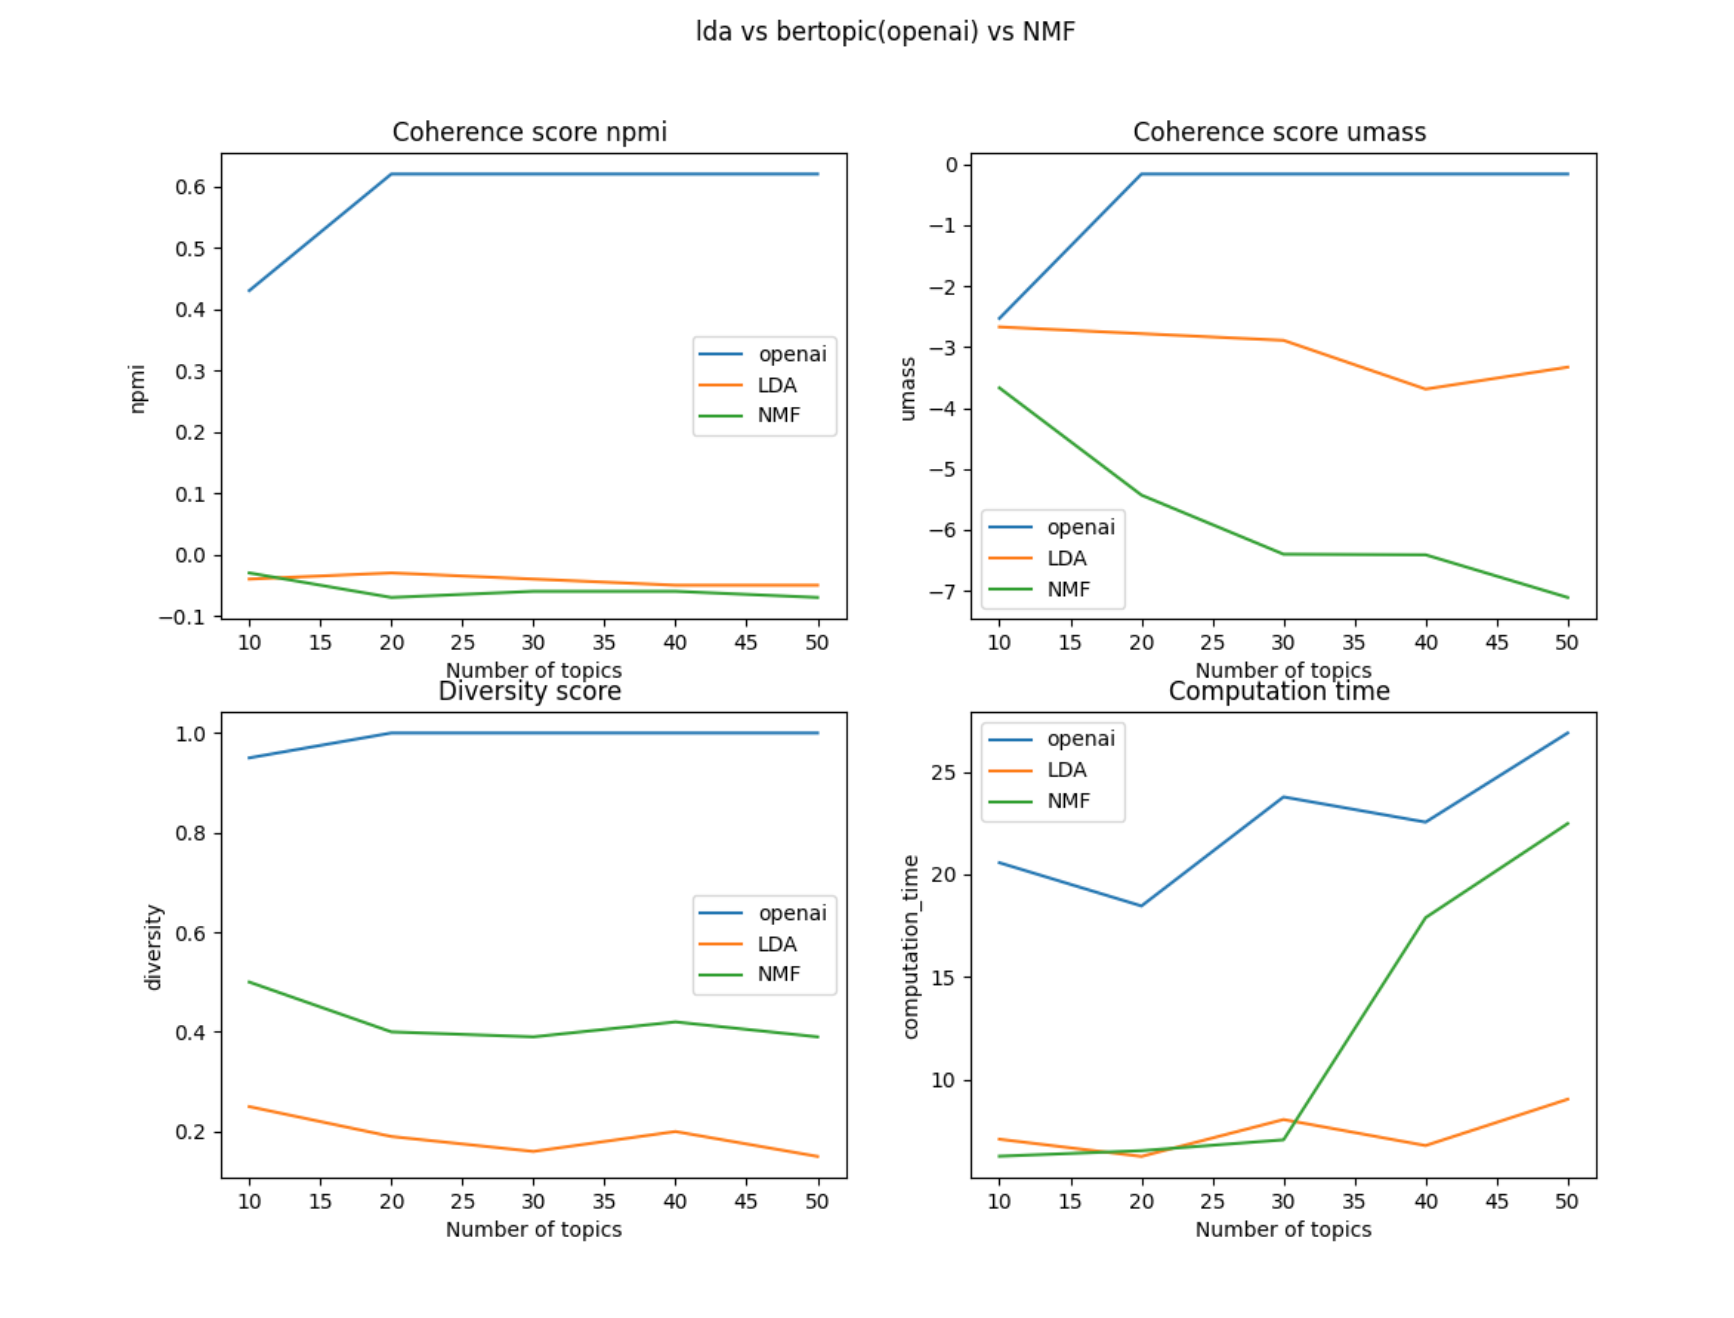
\includegraphics[width=0.99\linewidth]{Chapter4/figures/topic_unsupervised.png} 
    \caption{coherence and diversity for LDA, BERTopic, and NMF
    }
    \label{figure:unsupervised_results} % assign a unique label to each figure
\end{figure}


However, Hoyle et al  \cite{hoyle_is_2021} showed how these metrics are not very meaningful for evaluating these models and we should take these results with a grain of salt.

From this evaluation, we can conclude that for BERTopic the topic size is better bigger than smaller especially if we have many documents. Topics of Bertopic are way more diverse than LDA and NMF and within the topics, the most relevant word are more semantically related.


\subsection{Supervised}
Considering the result of the unsupervised evaluation we should use another method to validate what we found. In this case, we created two ad hoc datasets to see too how the models perform in a real-case scenario.

\paragraph{Dataset}

The first step for the supervised part was the data collection, in this case, we packed specific datasets to test our models. The first is simpler and contains very different topics so that should be easy to cluster the documents, while the second is more trickier because it contains only politics-related tweets with some overlapping.

\begin{itemize}
    \item \textbf{simple}: 1093 labeled tweets of 5 different topics identified by a hashtag \footnote{\#Bitcoin, \#stormydaniels, \#UkraineRussianWar, \#SaudiArabianGP, \#climatechange}
    \item \textbf{politics}: 1492 labeled tweets of 7 politics-related hashtags \footnote{\#IndictArrestAndConvictTrump, \#kabul, \#BidenHarris2024, \#KamalaHarris, \#taiwan, \#belarus,  \# stormydaniels}
\end{itemize}


For both datasets, we used two different versions: with and without hashtags.

The tweets have been extracted using \href{https://twarc-project.readthedocs.io/en/latest/twarc2_en_us/}{twarc2} getting only English tweets and without retweets.

\paragraph{Metrics}
In order to evaluate the topics we had to define some metrics:

\begin{itemize}
    \item \textbf{Accuracy}: for each known topic look at the biggest of inferred topics and divide by the number of tweets in that topic.
    \item \textbf{Accuracy no outliers}: in the Bertopic case the label -1 refers to outliers.
    \item \textbf{Min\_topic\_share}:  same as accuracy but in the opposite direction, after having computed it for all of my\_topics we take the minimum
\end{itemize}


\paragraph{Parameters}

\begin{verbatim}
BERTopic: (nr_topics = 'auto', min_topic_size = 50)

NMF: (max_df = 0.95, min_df = 3, ngram_range = (1,2))

GSDMM: (alpha = 0.1, min_df = 0.1, n_iters = 30)
\end{verbatim}


\paragraph{Simple Dataset Results}
We started evaluating the \textit{simple} dataset with hashtags and as we can see in Fig \ref{figure:supervised bar} base ( all-MiniLM-L6-v2) and OpenAi obtained almost a perfect score for each topic, while climatebert seems to have a great accuracy but a low mean topic share, this is a signal that something is wrong and we should inspect the heatmap.

\begin{figure}[h]
    \centering % figure is centered on the page
        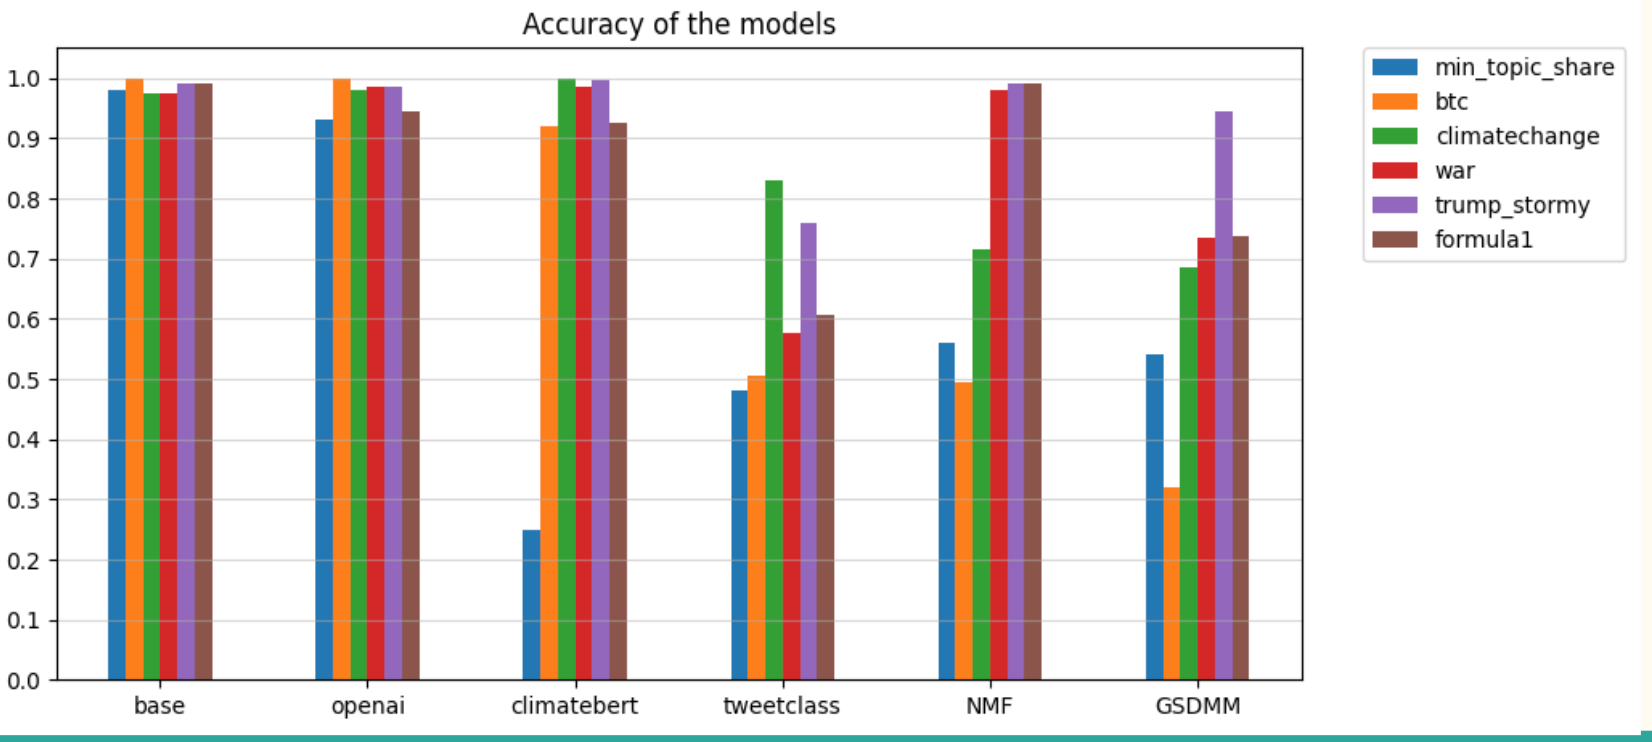
\includegraphics[width=0.99\linewidth]{Chapter4/figures/topic_supervised_bar.png} 
    \caption{All models accuracy simple  with hashtags
    }
    \label{figure:supervised bar} % assign a unique label to each figure
\end{figure}

In fact, we can clearly see in \ref{figure:sup_heatmap1_simple_hash} that even though the accuracy is very good, climatebert has some difficulties in dividing the topics putting almost all the tweets in the same. While the first two are performing very well as expected it is not true for the others. We can see how climate bert put almost all the tweets in topic 0, being able only to find the formula1 tweets and not the climatechange one, as it is designed to do.
That’s the reason why we decided to remove the models that are not performing well in the simplest case with the exception of NMF to use it as ground truth. 


\begin{figure}[h]
    \centering % figure is centered on the page
        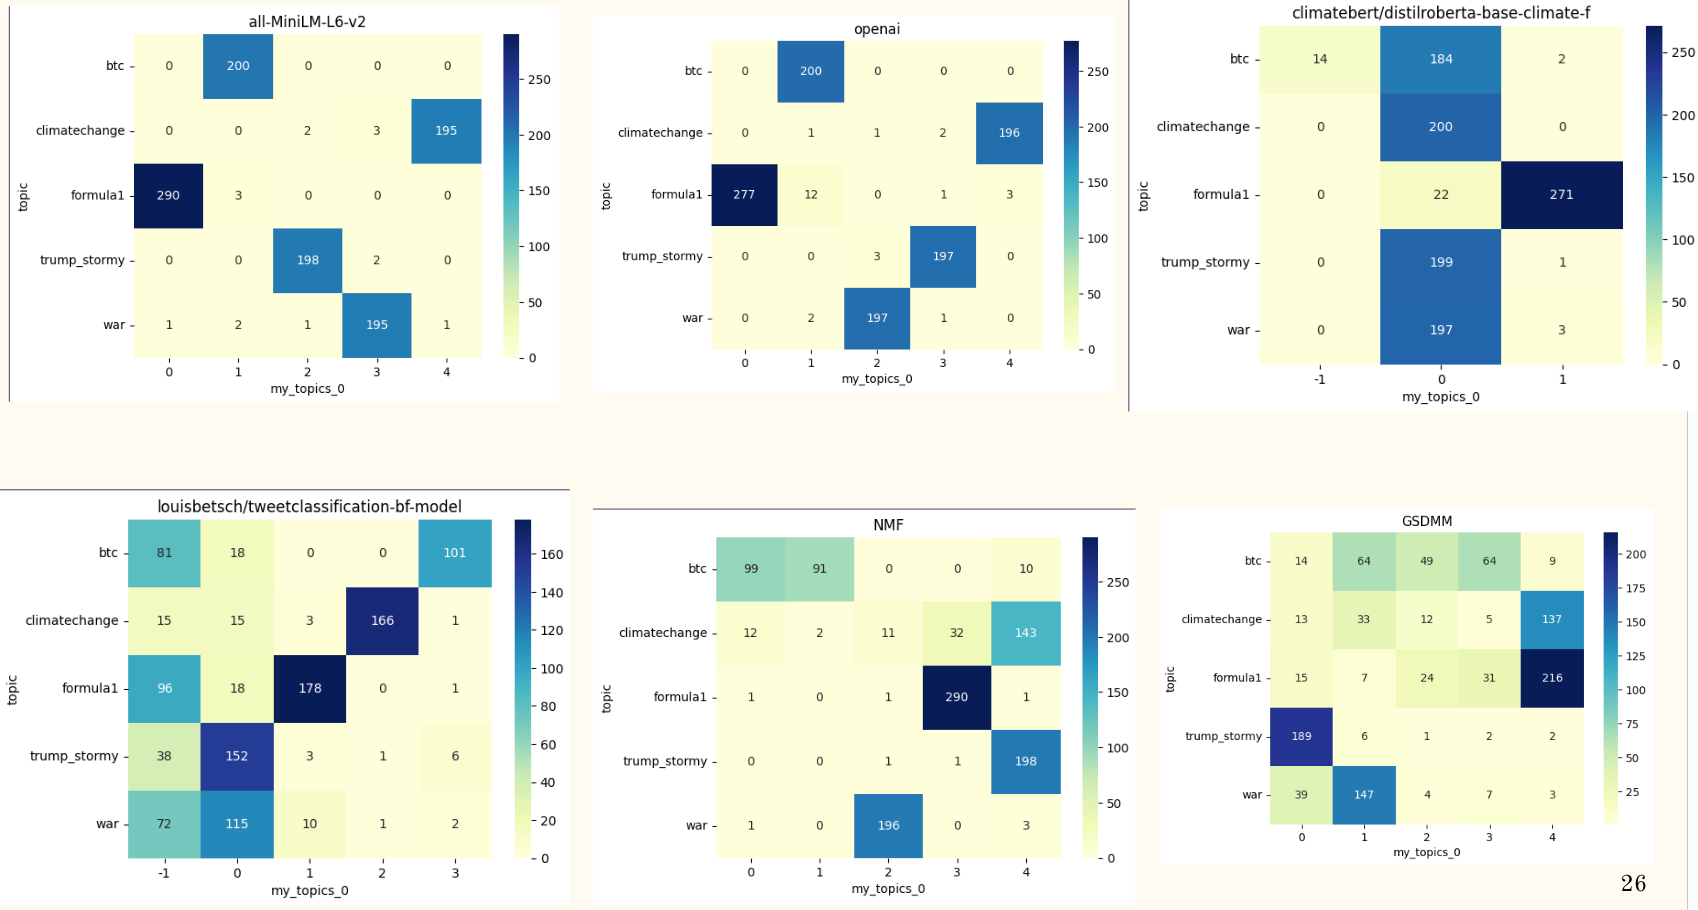
\includegraphics[width=0.99\linewidth]{Chapter4/figures/topic_heatmap1.png} 
    \caption{Heatmap comparison of the different model with the simple dataset with hashtags
    }
    \label{figure:sup_heatmap1_simple_hash} % assign a unique label to each figure
\end{figure}

Looking at \ref{figure:supervised heatmap1} we can see how BERT and OpenAI performed in the same dataset but without the hashtags, in particular how BERT tends to find more outliers than OpenAI.


\begin{figure}[h]
    \centering % figure is centered on the page
        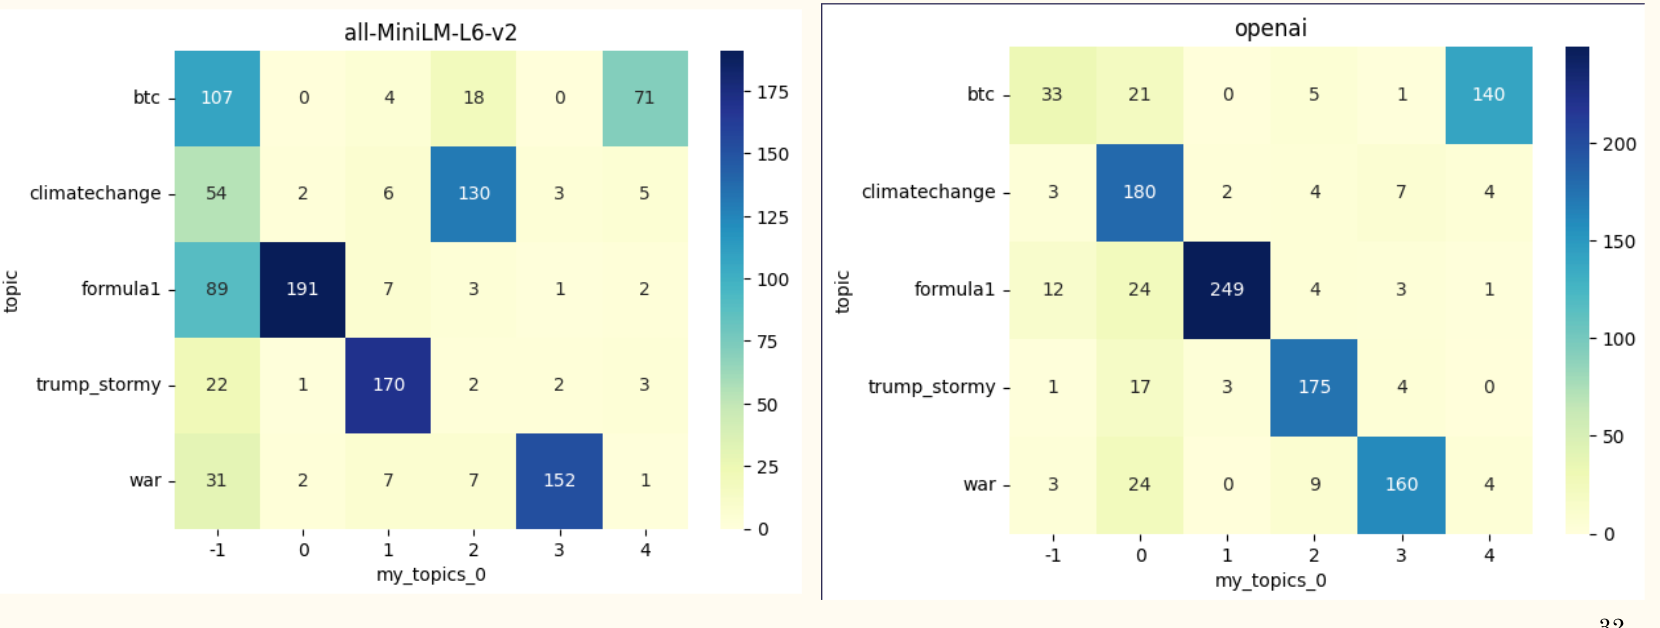
\includegraphics[width=0.99\linewidth]{Chapter4/figures/topic_heatmap_bertopic.png} 
    \caption{Heatmap comparison of mini and OpenAi of the simple dataset without hashtags}
    \label{figure:supervised heatmap1} % assign a unique label to each figure
\end{figure}
An interesting feature of Bertopic is the ability to visualize the different topics in a 2-dimensional space, Fig \ref{fig:openai docs} show the document distribution of OpenAi after projecting the embeddings in a two-dimensional space.
\begin{figure}
    \centering
    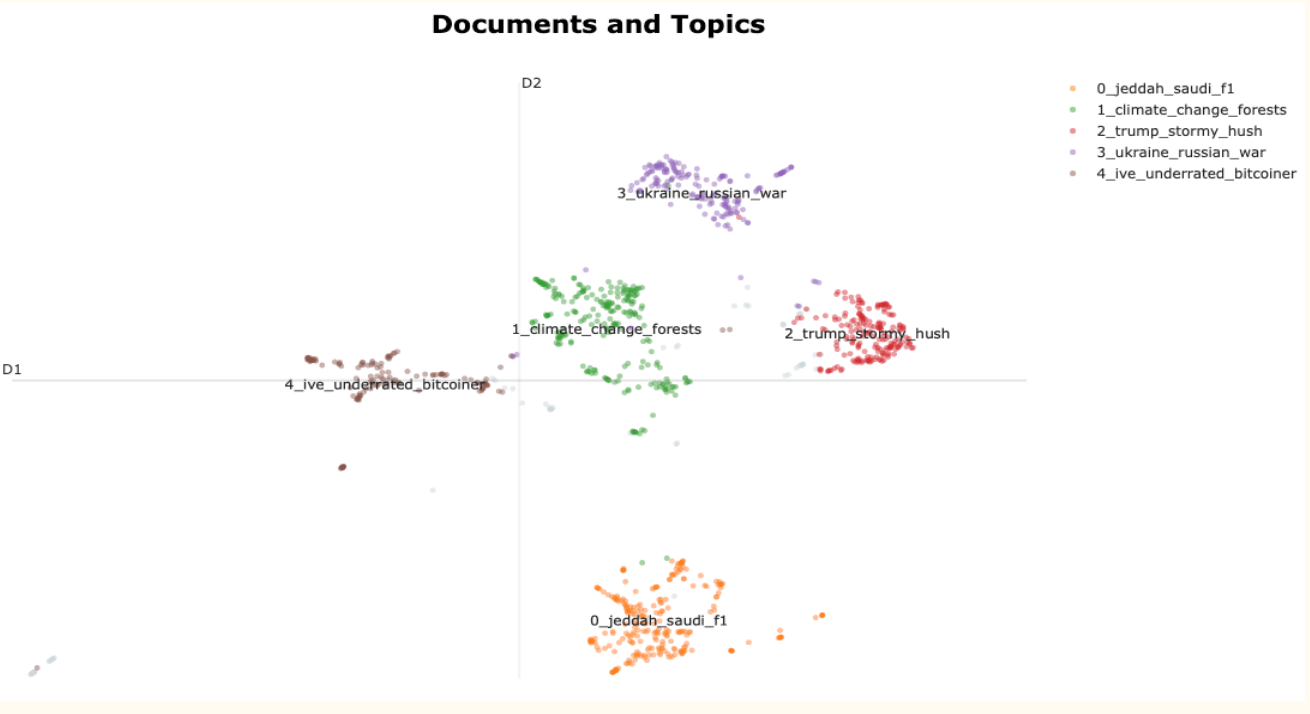
\includegraphics[width=1\linewidth]{Chapter4/figures/openai_documents_viz.png}
    \caption{docs representation of simple dataset for openai}
    \label{fig:openai docs}
\end{figure}


\paragraph{Politics dataset results}

The politics dataset is clearly more difficult to evaluate but with the hashtags it is still doing a good job. Even though we can see that both BERT and OpenAi are merging two topics. In particular, for OpenAi makes more sense since the two hashtags related to Trump are related to the same event( \#trump and \#trump\_stormy

\begin{figure}
    \centering
    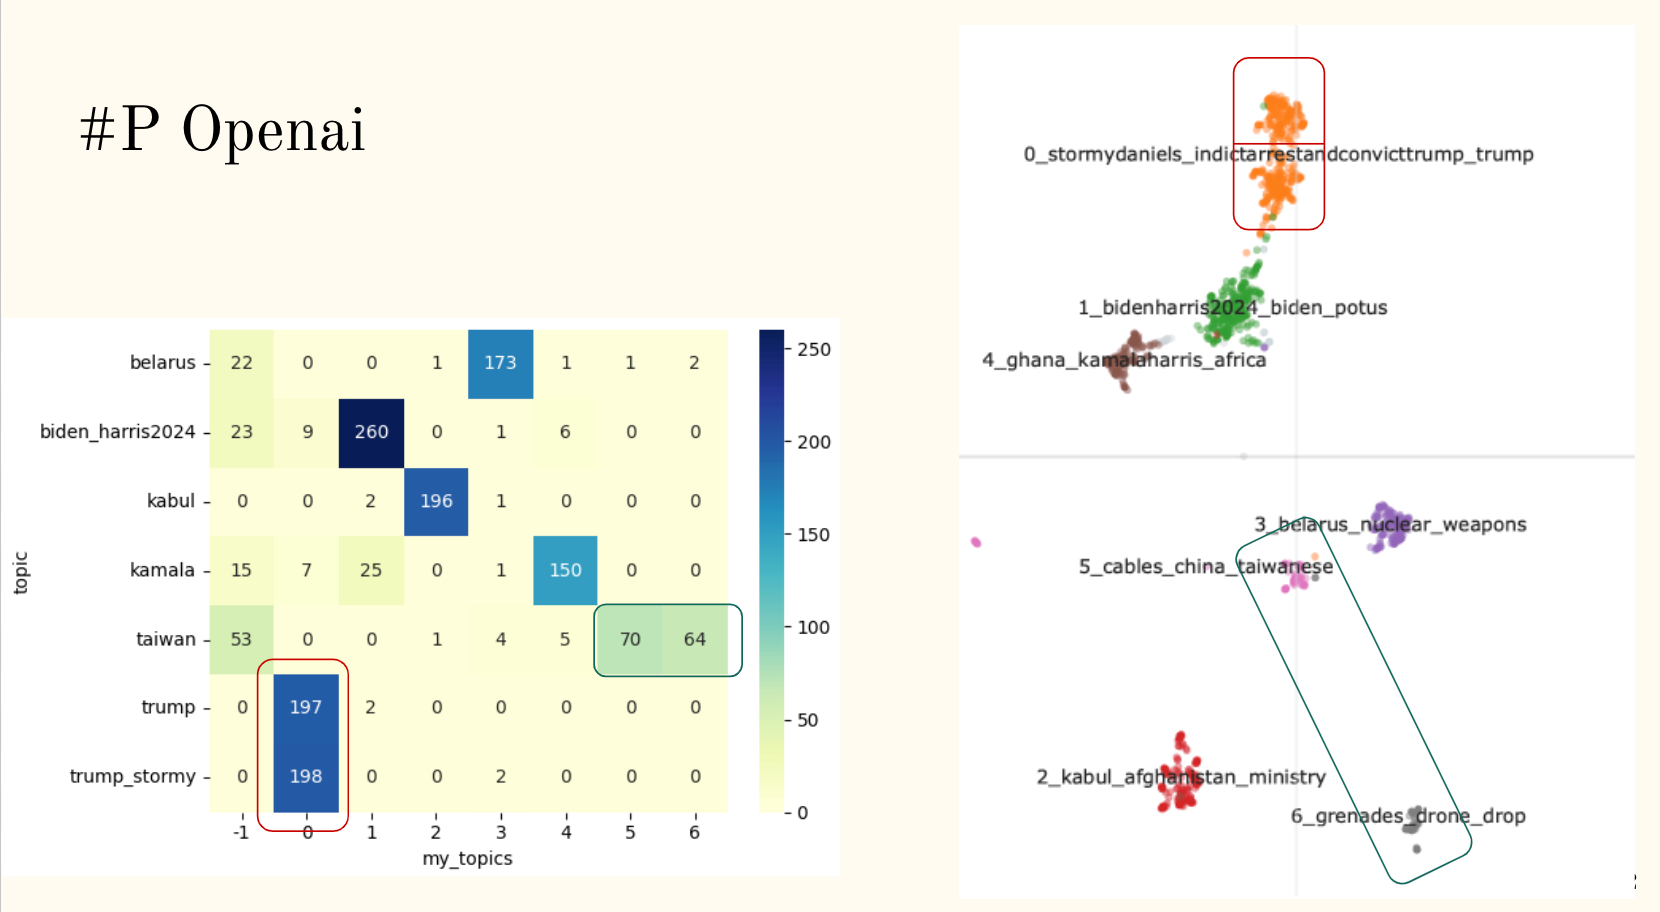
\includegraphics[width=1\linewidth]{Chapter4/figures/openai_politics_hash_comparison.png}
    \caption{Heatmap and documents representation of the politics dataset with hashtags evaluated with openai}
    \label{fig:openai_heat_docs_politics_hash}
\end{figure}

To validate the results we run the algorithm 100 times and most of the time for BERT the min topic share is 0.9 which means they got the correct number of topics and classified them in a good way. We can look at Fig \ref{fig:bert politics with hashtags} to see both documents and the heatmap.

\begin{figure}
    \centering
    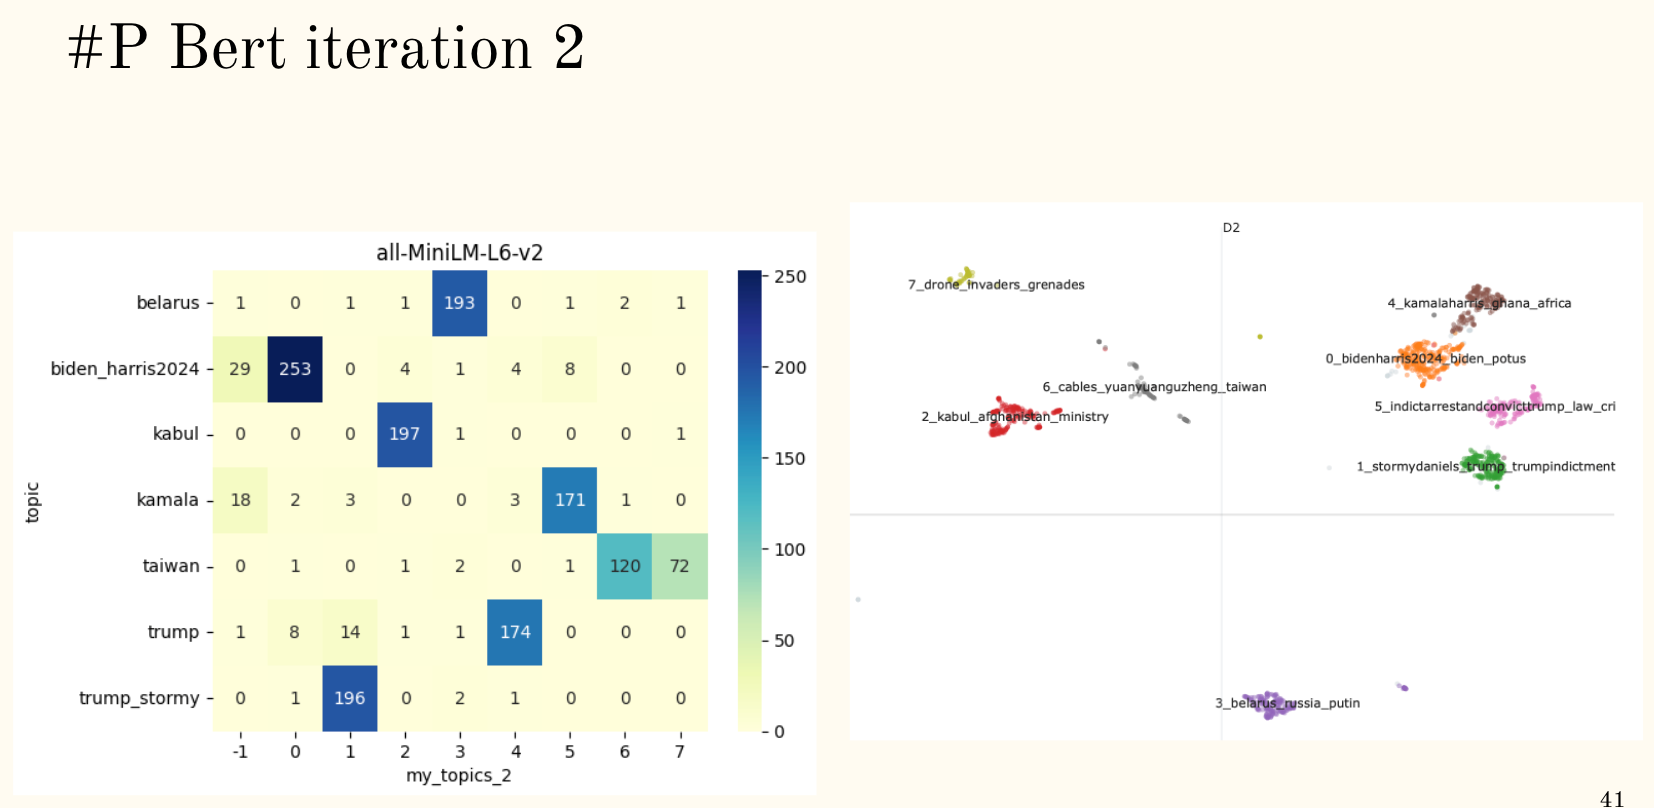
\includegraphics[width=1\linewidth]{Chapter4/figures/bert_politics_hash_comparison.png}
    \caption{bert heatmap and document viz politics with hashtags}
    \label{fig:bert politics with hashtags}
\end{figure}
in the case without hashtags OpenAi and BERT put in a single cluster all the tweets related to American politics both also understanding that Kamala's tweets were about something else.

\paragraph{Conclusion}
Tab \ref{tab:unsupervised_recap} show the result of unsupervised evaluation, while Tab \ref{tab:supervised recap } the supervised


\begin{table}[]
\centering
\begin{tabular}{|llll|}
\hline
\textbf{model}                              & \textbf{npmi} & \textbf{umass} & \textbf{diversity} \\ \hline
\multicolumn{1}{|l|}{tweet\_classification} & 0.62          & -0.16          & 1                  \\
\multicolumn{1}{|l|}{openai}                & 0.58          & -0.63          & 0.99               \\
\multicolumn{1}{|l|}{climatebert}           & 0.20          & -2.28          & 0.83               \\
\multicolumn{1}{|l|}{U.S.E}                 & 0.20          & -4.35          & 0.89               \\
\multicolumn{1}{|l|}{BERT}                  & 0.20          & -5.46          & 0.97               \\
\multicolumn{1}{|l|}{LDA}                   & -0.04         & -3.07          & 0.19               \\
\multicolumn{1}{|l|}{NMF}                   & -0.06         & -5.80          & 0.42               \\ \hline
\end{tabular}
\caption{all the models tested in the unsupervised evaluation}
\label{tab:unsupervised_recap}
\end{table}

\begin{table}[]
\centering
\begin{tabular}{|l|ll|}
\hline
model  & accuracy & topic share \\ \hline
BERT   & 0.84     & 0.86        \\
OpenAI & 0.83     & 0.85        \\
NMF    & 0.78     & 0.69        \\ \hline
\end{tabular}
\caption{recap of supervised evaluation}
\label{tab:supervised recap }
\end{table}




\section{Multilayer Network}

In this section, the analysis will dive into all the unexplored paths, starting from Falkenberg’s work. In particular, the same polarization analysis will be conducted on a topic level: instead of computing it at a full network level, a retweet network was created for each topic, so the topics that were driving the polarization of cop emerged. Furthermore, the aim was also  to explore how the polarization of topics evolved over time.

By reading the previous section, the concept of topic modeling is known, and so is the way the main models perform. The goal is to create a multilayer network where every layer represents a topic.

In order to do so, a Python library was developed, which can be used as a toolbox, starting from the tweets fresh out from the official API of Twitter. The design is modular and can achieve different goals. In fact, even if the  interest is only in the retweet network of the users (nodes are users, ties are retweets), this framework can be used to perform different tasks, but to the purpose of this study the tasks highlighted are: 

\begin{itemize}
    \item Clustering tweets according to their topic
    \item Giving a meaningful label to the clusters
    \item Creating the retweet network (global and multilayer version)


\end{itemize}

The steps are independent, so, for example, it is possible to create the network without the need to run the topic modeling part.


\paragraph{Steps}
Even though some steps are avoidable, the natural and minimal pipeline follows these steps:


\begin{enumerate}
    \item from JSON to a tabular format 
    \item label each tweet with a topic
    \item create multilayer retweet network  
    
\end{enumerate} 


\subsection{Process input}

The first step consists of the transformation of the JSON objects into tabular data to optimize the space and handle the data in an easier way with pandas. This is also helpful to save space; in the case of COP26, a shift is made from a 14 GB JSON to a less than 2 GB CSV, since most of the fields are not relevant to this study.

In this process, all the tweets with attachments and not in English are discarded. The tweets are divided into multiple dataframes: one for original tweets - i.e., the ones that the author actively writes-, and one for the retweets.

At the end of this stage, a CSV and pkl file are saved in case somebody needs the tweets in tabular data. If the script is re-run and these files exist, they will be loaded instead of running the process again.


\subsection{Topic modeling}

As extensively discussed in chapter 2, in this segment of the pipeline the tweets can be labeled using Bertopic, with the possibility to choose the embedder; the one used in this research is\textit{ all-MiniLM-L6-v2}, the one evaluated in the previous section.

This step is the most computationally expensive; for this reason, to avoid redundancy, the topic modeling has been run only using original tweets.


After this step, all the original tweets are labeled with a numeric topic, and then the label has been propagated to all the retweets so that the entire dataset is now labeled with a topic.

At this point, the OpenAI API can be used to give a meaningful label to the topics, while beforehand, the labels were just made of the most relatively frequent words of the topic. By using the langchain library, it is possible to structure an employable  prompt. The model was assigned the words identified with TF-IDF and 3 representative tweets sampling a subset of the documents in each topic, and calculated on the cosine similarity between TF-IDF representations.


This is the one used: 
\\

\textit{    I want you to act as a tweet labeler, you are given representative words
from a topic and three representative tweets, give more attention to the words, all the tweets are related to climate change and COP, there is no need to mention them, detect subtopics.
start with "label:" and avoid hashtags,
which is a good short label for the topic containing the words [{words}]?, here are 3 tweets to help you:
first = "{tweet1}", second = "{tweet2}", third = "{tweet3}}
\\

Similarly to the previous stage, the labeled dataset is saved in the cache folder both in CSV and pkl. The model and the labels are saved, too.



\subsection{Network}
In this phase, after labeling the tweets, a retweet network will be created for each topic, gathering it all together in a multilayer network.
%The network is directed, the nodes are the users, and the tie is the number of retweets. For each topic, a network is created.

In the process of the creation of the network, there are retweeted tweets that do not have the original one, so they are  discarded.

The last step is the creation of a multilayer network using the multinet library developed by Uppsala University; Every layer is a retweet network of a specific topic. It was built starting from the subset of tweets of a specific topic, the unique users are the nodes and, if user A retweets user B there will be a tie $A \rightarrow B$. The network is directed and weighted with the number of retweets. Fig \ref{fig:multilayer} is a simple example of a network with 2 layers.

The network then has been filtered by removing the outlier layer, labeled with -1.

\paragraph{COP26 network}
For COP26, 70 layers were detected, the average number of users per layer is 8127, min is 15, max is 108829,

\paragraph{COP21 Network}
For COP26, 36 layers were detected, the average number of users per layer is 10123, min is 696, max is 142062,



\begin{figure}
    \centering
    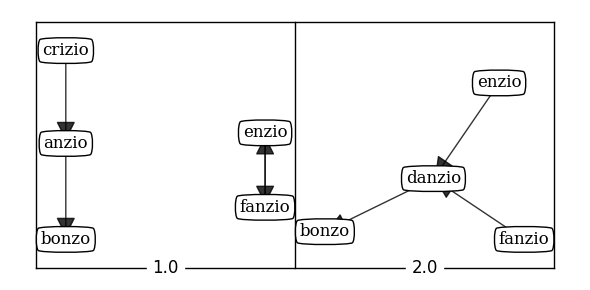
\includegraphics[width=0.75\linewidth]{Chapter4/figures/projected_topics_ml.png}
    \caption{Example of multilayer retweet network }
    \label{fig:multilayer}
\end{figure}




\section{Polarization}
At this point, for each layer, it is possible to compute for each user a latent ideology score, and then, using Hartigan’s diptest, a polarization value  can be assigned to each topic. More details on how this is computed are dealt with in the related works. In this process, there are some parameters that can be adjusted: the number of influencers - defined as the most retweeted users-, and $n$ - representing the minimum number of retweets a user should have made to an influencer to be considered-.

The ideology score is not computed on all the users, but when selecting the influencers, the users are limited to the ones that retweeted at least n times those influencers.

In order to have enough data to be analyzed, the values set were $n\_influencers = 100$ and $n=2$. The hartigan diptest requires a minimum of nodes to be statistically significant and, since at this point the layer are filtered, all the layers with a p-value of the diptest higher than 0.05 have been discarded.


\paragraph{COP26 }
The number of networks goes from 70 to 30 . The total influencers considered in the analysis of COP26 is 1698. 22302 users have an assigned score for cop26, with an average of 1311 actors per topic, with a min of 151 and a max of 7764.

\paragraph{COP21}
the number of networks went from 36 to 8. The total number of influencers considered in the analysis of COP21 is 392. 8020 users have an assigned score, with an average of 2058 actors per topic, with a min of 35 and a max of 7524. 

Tab  \ref{tab:recap_ideology} presents a summary of the starting networks 


\begin{table}[h]
    \centering
    \begin{tabular}{|l|l|l|l|}
        \hline
        \textbf{Description} & \textbf{COP21} & \textbf{COP26} & \textbf{COP2x}\\ \hline
        Initial topics & 36 & 70 & 54 \\ \hline
        Final topics & 8 & 26 & 29\\ \hline
        Influencers scored & 392 & 1557 & 1559\\ \hline
        Users scored & 8020 & 22161& 33312 \\ \hline
        Mean users/topic &  2058 & 1311 & 1766\\ \hline
        Min users/topic & 35 & 151 & 123\\ \hline
        Max users/topic & 7524 & 7764 & 14504\\ \hline
        diptest &1 & 0.07 & 0.05 \\ \hline
        \end{tabular}
        \caption{Summary of Latent ideology}
    \label{tab:recap_ideology}
\end{table}


\section{Logitudinal analysis}
In order to see topic polarization over time, we need to run the topic modeling with all the tweets. Still, there are too many, so instead of taking the original tweets of COP21 and COP26, we only take the original with at least one retweet which are around 1/3 of the total but are the one needed to create  the rest of the network.

Then the two dataset have been merged, we will refer to this dataset $COP2x$ and the same process described below has been done.




 

\chapter{Results}%Or Results
\label{ch:res}
Let us start drawing a big picture of the different topics that emerged after the latent ideology analysis. 


Fig \ref{fig:diptest} summarize the size of the newtorks and the diptest result, so the polarization, for each topic. The first thing to note is the fact that to the highest polarization corresponds the smaller topics, with the exception of topic 14. For the first two topics the polarization is significantly higher than the others.


\begin{figure}[H]
    \centering
    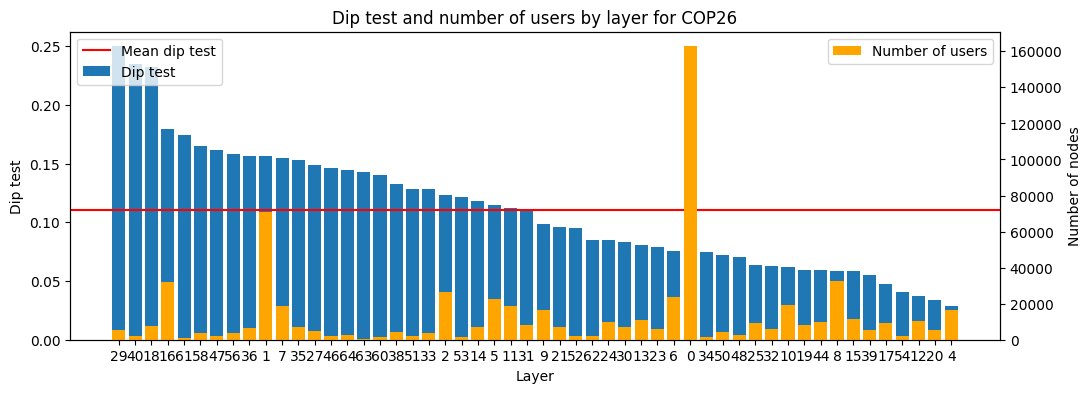
\includegraphics[width=0.95\linewidth]{Chapter5//figures/diptest_cop26.png}
    \caption{Dip test and number of users for cop26 topic by topic}
    \label{fig:diptest}
\end{figure}

\section{RQ1 Most Polarized Topics}


Fig \ref{fig:networks_polarization} let us visualize the most and the least polarized topics, every network represent the retweet network of the 100 biggest influencers, in the leftmost plot we can find the full network while in the rightmost only the influencers are present. In the most polarized topics we can clearly see how the influencers are almost equally split between the two poles. Falkenberg it its work identified a majority of pro climate and a minority of climate skeptics, but looking at a topic level we can see how the two groups are equally split, and the networks that present the majority-minority dicotomy are the least polarized. A notable example is the most polarized topic: "Canada Climate Change goals" which refers to the announcement of Canada's first minister to cap gas and oil emissions. This decision caused many disagreement, in Tab \ref{tab:canadatweets} some random tweets against the decision, user 1 argument that this will destroy the economy, user 2 instead is generally against all the decision of Trudeau, as states in her biograpahy : "Lover of gardening, antiques and anyone who wants to see the end of the Trudeau government." This  follows the typical elite polarization pattern, where political exponent strictly adhere to their party policies, in this case it is not a political party but a politically-aligned individual which is, in some way, forced to follow her self-imposed guidelines in her biography to avoid cognitive dissonance \cite{Festinger_dissonance_57}.

\begin{table}[]
\centering
\begin{tabular}{|p{1in}|p{4in}|}\hline
\textbf{user} & \textbf{tweet} \\ \hline
User1     & This meme could just as easily apply to Canada. Trudeau’s willingness to destroy our economy to the benefit of others is akin to cutting off our noses to spite our faces!\%. \\ \hline
user2        & \#COP26 Maybe some people are still fooled by Justin Trudeau and his dishonest climate change stories, but there are plenty of us here in Canada who are not. Look into the truth about the Lytton fire. It won't come out of Justin Trudeau's mouth \\ \hline
user3          & Capping emissions in the country while exporting oil, gas and coal out of the country. Hypocrisy.
 \\ \hline
\end{tabular}
\caption{}
\label{tab:canadatweets}
\end{table}




It is interesting to note in Fig \ref{fig:ridge_topics} the distribution of the tweets of each topics over time during the cop, the dotted line marks the start end end date of COP26. The most polarized had interest only in few days losing quickly the interest. The opposite happens in the least polarized topics where the discussion is distributed over a longest timespan.  



\begin{figure}[H]
    \centering
    \begin{minipage}{0.50\textwidth}
        \centering
         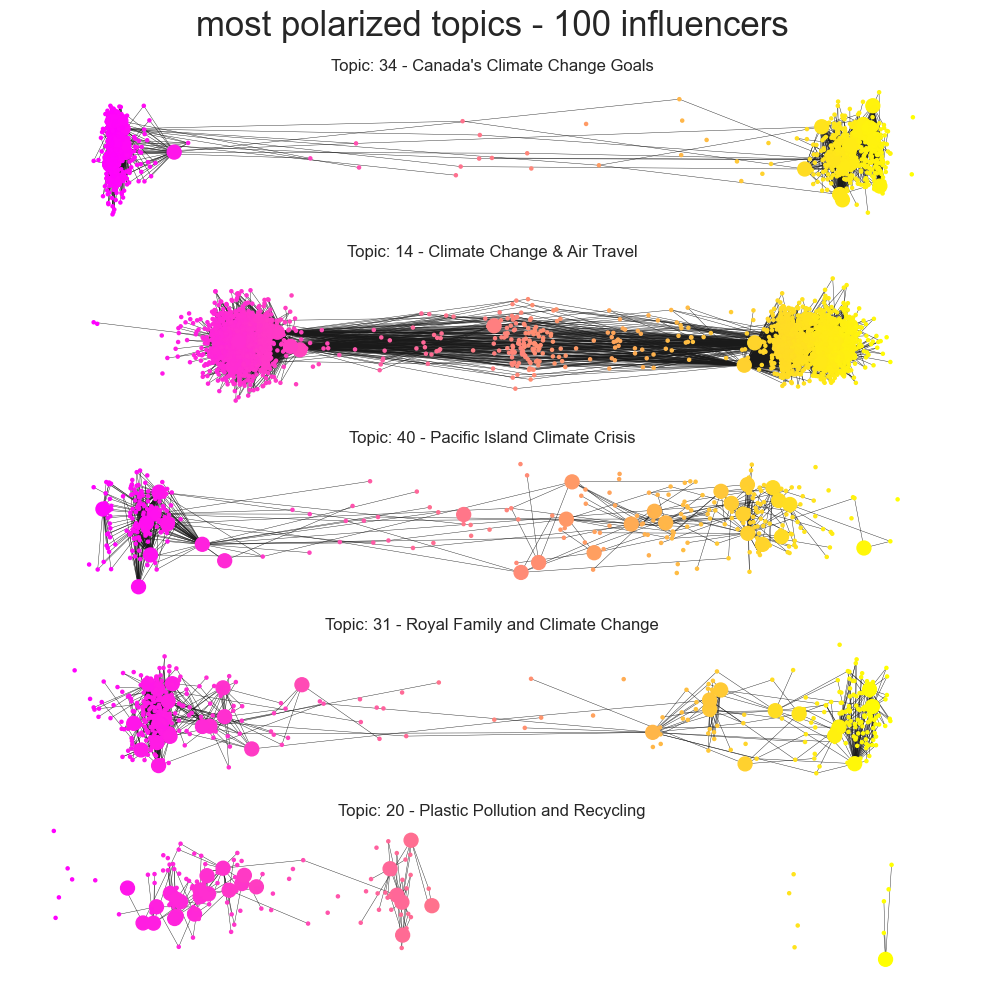
\includegraphics[width=0.98\linewidth]{Chapter5//figures/most_pol_cop26.png}
        \caption{most polarized topics}
    \end{minipage}\hfill
    \begin{minipage}{0.50\textwidth}
        \centering
         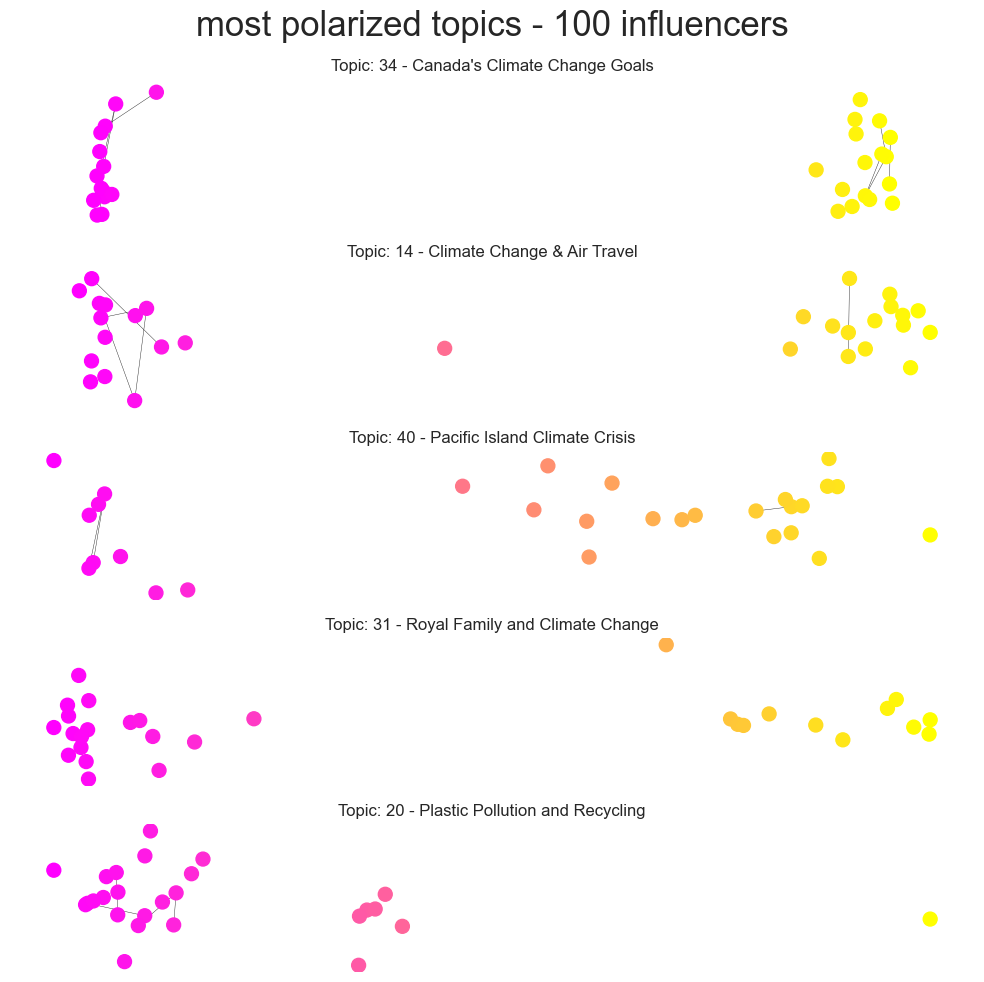
\includegraphics[width=0.98\linewidth]{Chapter5//figures/most_pol_cop26_inf.png}
        \caption{most polarized topics only infleuncers}
    \end{minipage}
    \begin{minipage}{0.50\textwidth}
        \centering
         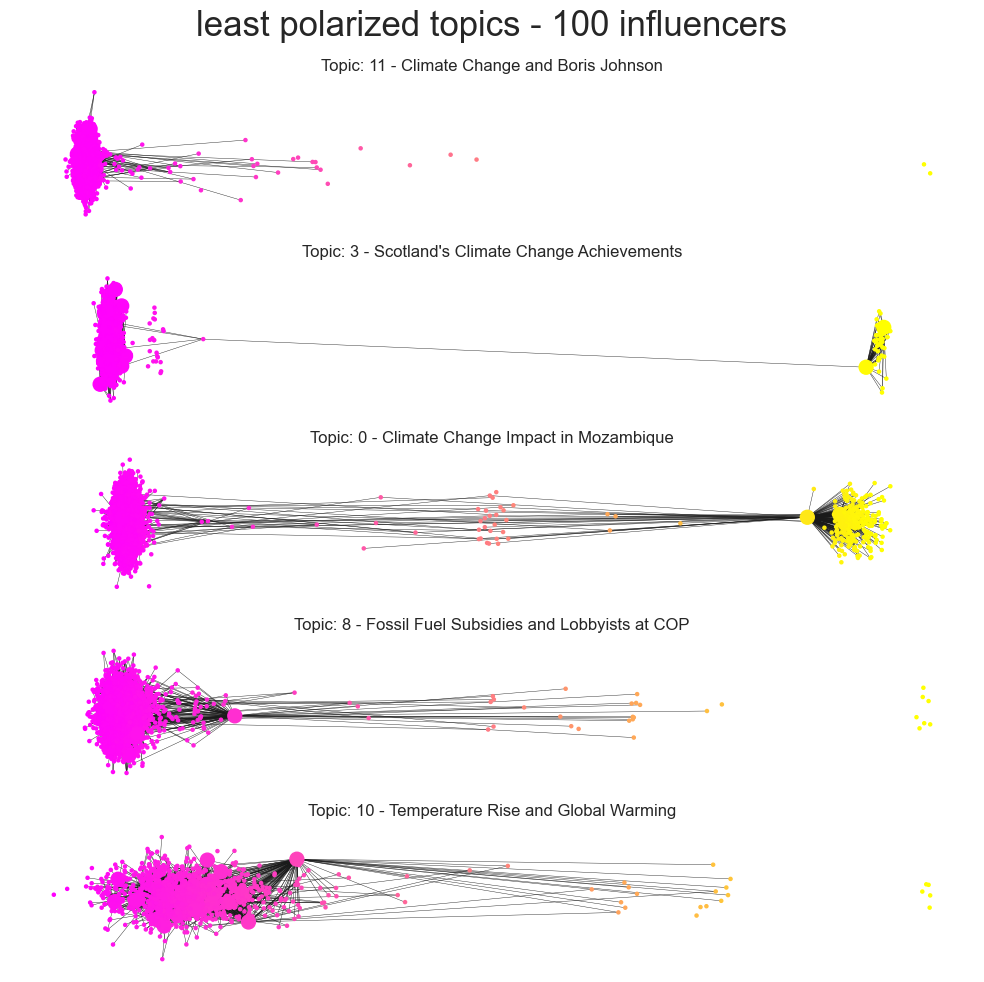
\includegraphics[width=0.98\linewidth]{Chapter5//figures/least_pol_cop26.png}
        \caption{least polarized topics}
    \end{minipage}\hfill
    \begin{minipage}{0.50\textwidth}
        \centering
         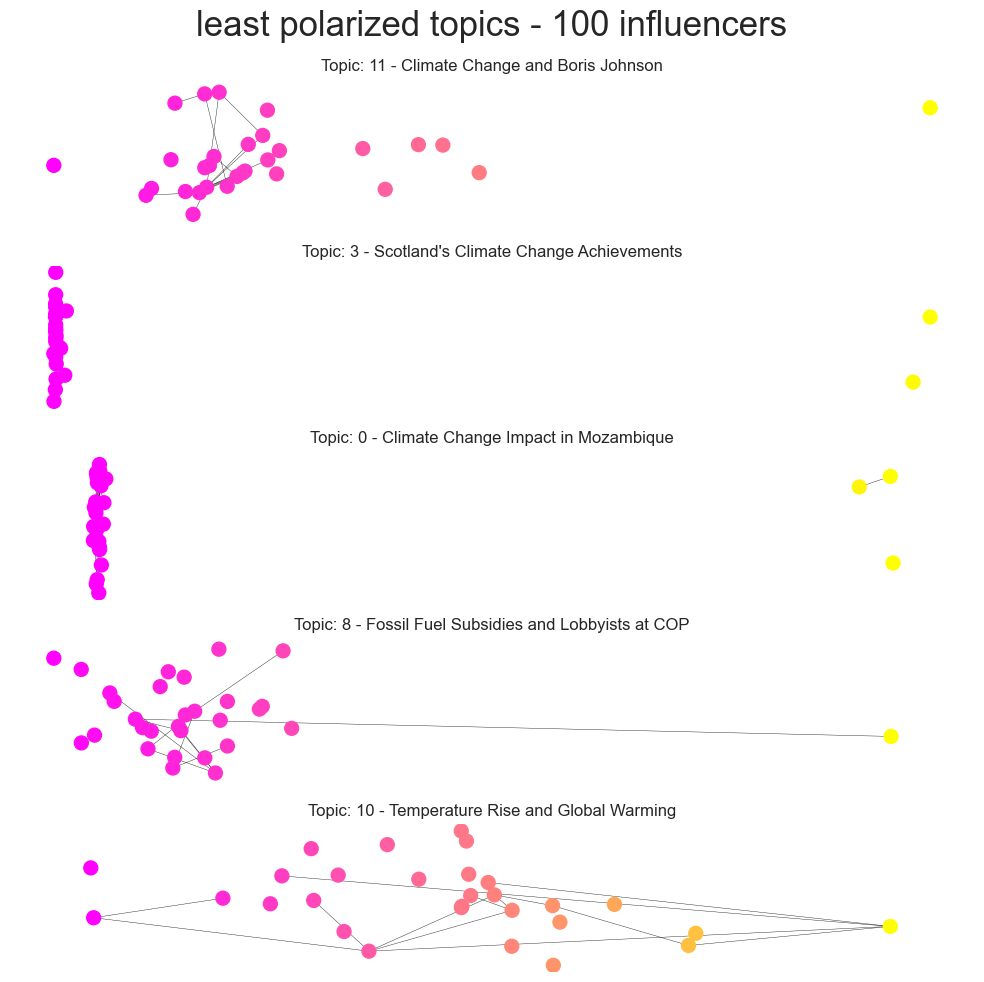
\includegraphics[width=0.98\linewidth]{Chapter5//figures/least_pol_cop26_inf.png}
        \caption{least polarized topics only influencers}
    \end{minipage}

    \caption{least and most polarized topics}
    \label{fig:networks_polarization}
\end{figure}


\begin{figure}[H]
    \centering
    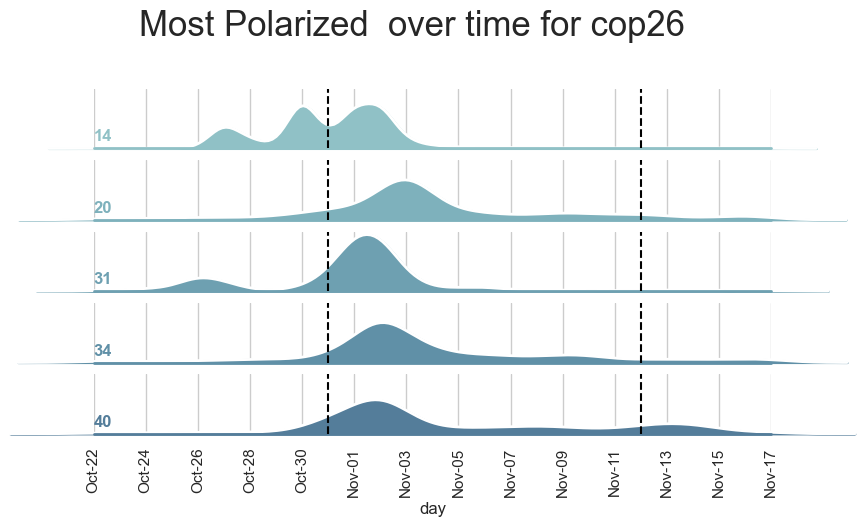
\includegraphics[width=0.75\linewidth]{Chapter5/figures/ridge_most_26.png}
     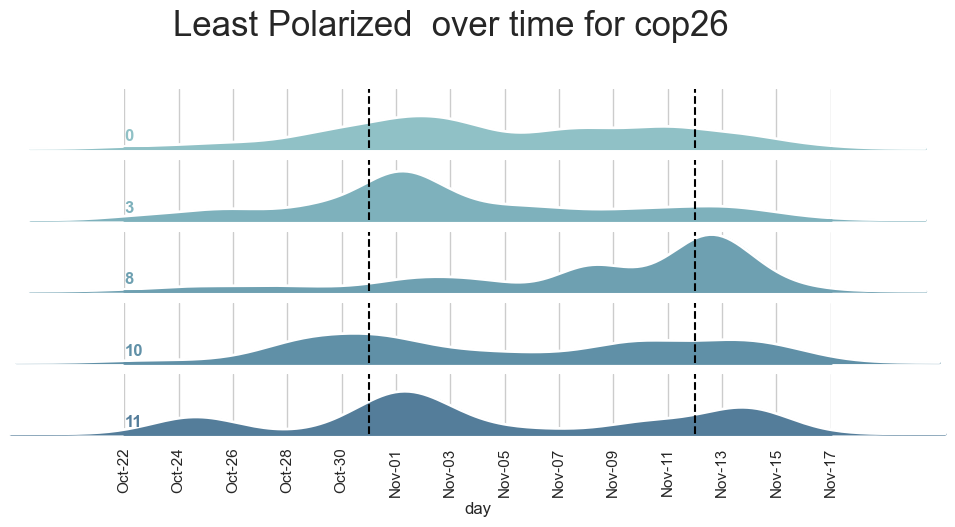
\includegraphics[width=0.75\linewidth]{Chapter5/figures/ridge_least_26.png}
    \caption{Enter Caption}
    \label{fig:ridge_topics}
\end{figure}


\section{RQ2 Longitudinal analysis}

In this section we compare the polarization between cop21 and cop26, to do so, we had to run the topic modeling together, in Fig \ref{fig:diptesto cop2x} the diptest results is shown, here we can find a similar trend of the cop26, the biggest topics are less polarized, with the exception of topic 9. Fig \ref{fig:2126_share} helps understanding the share of the tweets between cop21 and cop26. We can see how topic 9 which is the most polarized is composed mostly by tweets from cop26, which is aligned with the literature. Now we will look into some topics, creating the network if retweets both for bot COPs and we will compare them. We can compute this analysis only on topic 1,3 and 12 which are the ones that are polarized and have enough tweets in bot cops to run latent ideology.  

\begin{figure}[H]
    \centering
    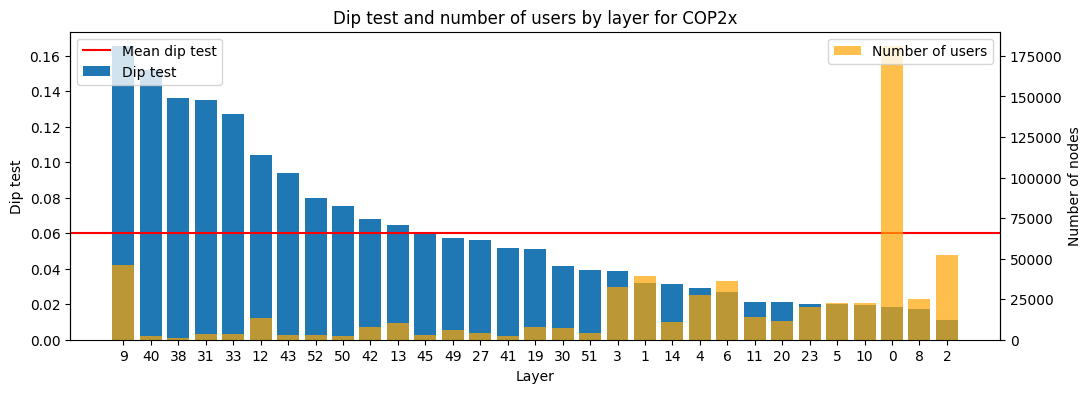
\includegraphics[width=0.8\linewidth]{Chapter5//figures/diptest_cop2x.png}
    \caption{Enter Caption}
    \label{fig:diptesto cop2x}
\end{figure}

\begin{figure}[H]
    \centering
    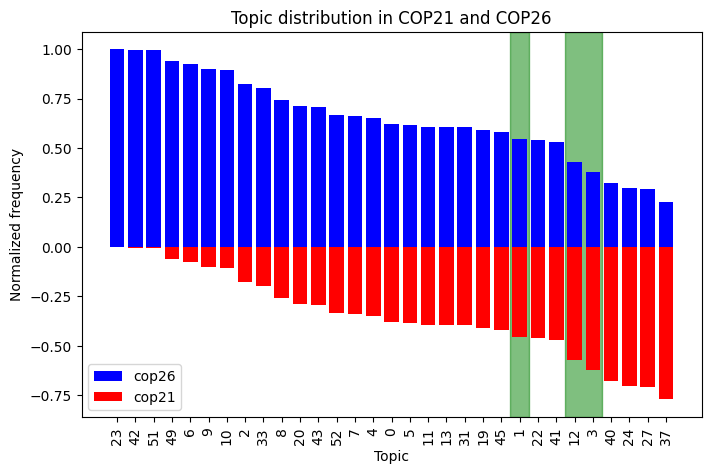
\includegraphics[width=0.8\linewidth]{Chapter5/figures/cop21vscop26.png}
    \caption{Enter Caption}
    \label{fig:2126_share}
\end{figure}

Fig \ref{fig:cop2x_network_comparison} show the results of this analysis. It is worth noting how topic 12 is the topic talking about Canadian fossil fuels, discussion that was present in both cops, but with a very different level of polarization. Overall the results confirm the hypotesis that cop26 is more polarized of cop21, but these are just three topics, to confirm this we should run the same analysis with more data.

\begin{figure}[H]
    \centering
    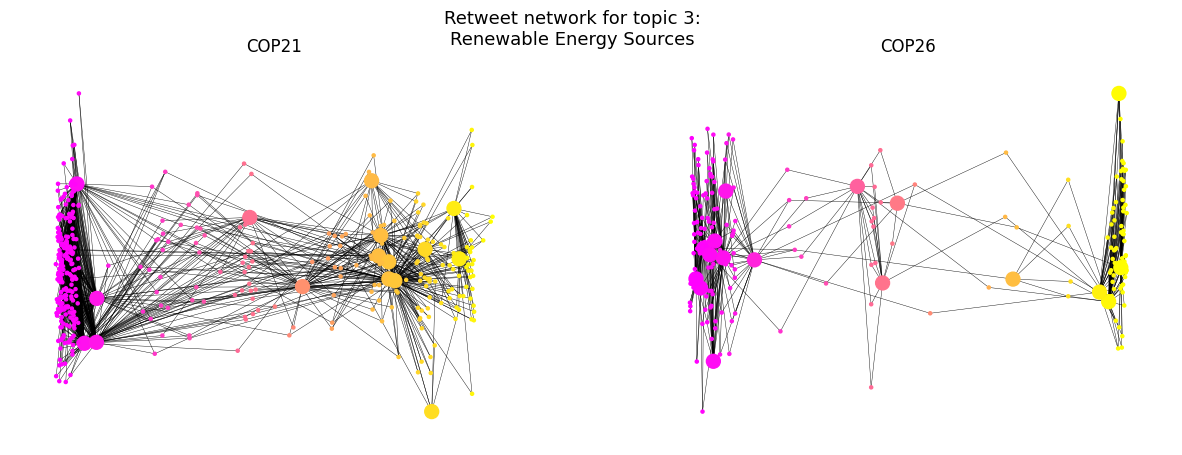
\includegraphics[width=0.95\linewidth]{Chapter5//figures/21vs26_t3.png}
    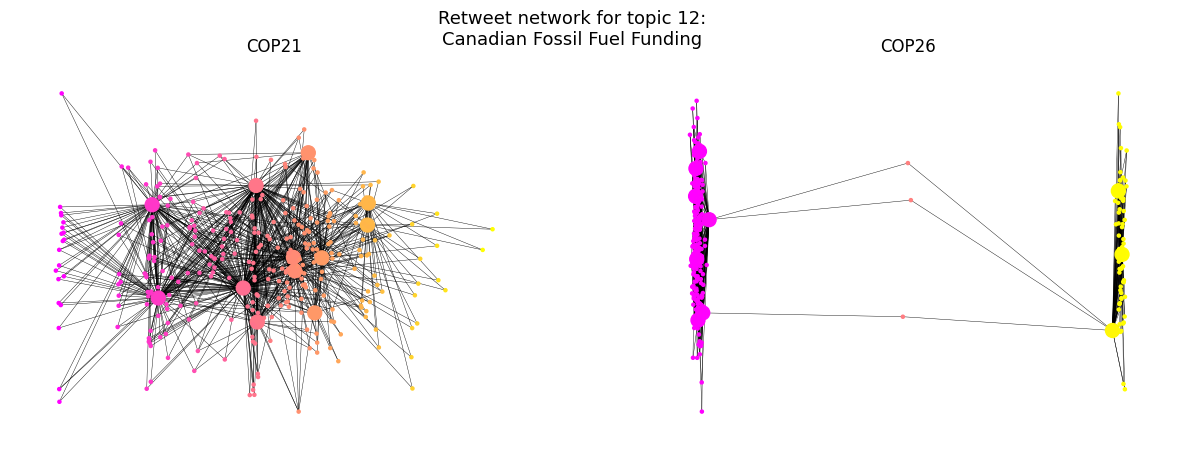
\includegraphics[width=0.95\linewidth]{Chapter5//figures/21vs26_t12.png}
    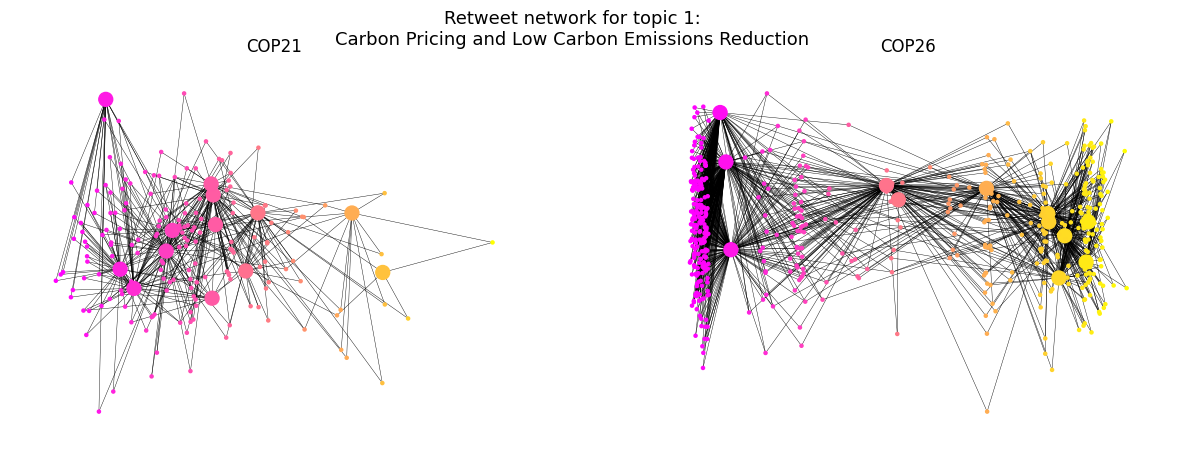
\includegraphics[width=0.95\linewidth]{Chapter5//figures/21vs26_t1.png}
    \caption{Enter Caption}
    \label{fig:cop2x_network_comparison}
\end{figure}

\section{RQ3 User polarization among different topics}
After computing the polarization score for all users we can now analyze whether the the users are polarized in the same way among all the topics they were active in.

The number of users involved in this analysis is 22161 active in 26 topics. most of them (16141) were only active in one topic, the maximum is 23 and the average is 1.53 topics per user. 

Then we computed, for each user present in more than 1 topic, the average and the standard deviation of the score. This value is higher for the users that are present in both side of the spectrum so this allow us to identify the degree to which users tend to be monopolar.

Fig \ref{fig:std_avg} show how the distribution of the average score for every topic aggregated together, this matches with the global results of Falkenberg, where a majority is present on the $-1$ side versus a minority in the $1$ side.

In the std we can see how there is a strong tendency to stay in the same side of the spectrum.

\begin{figure}[H]
    \centering
    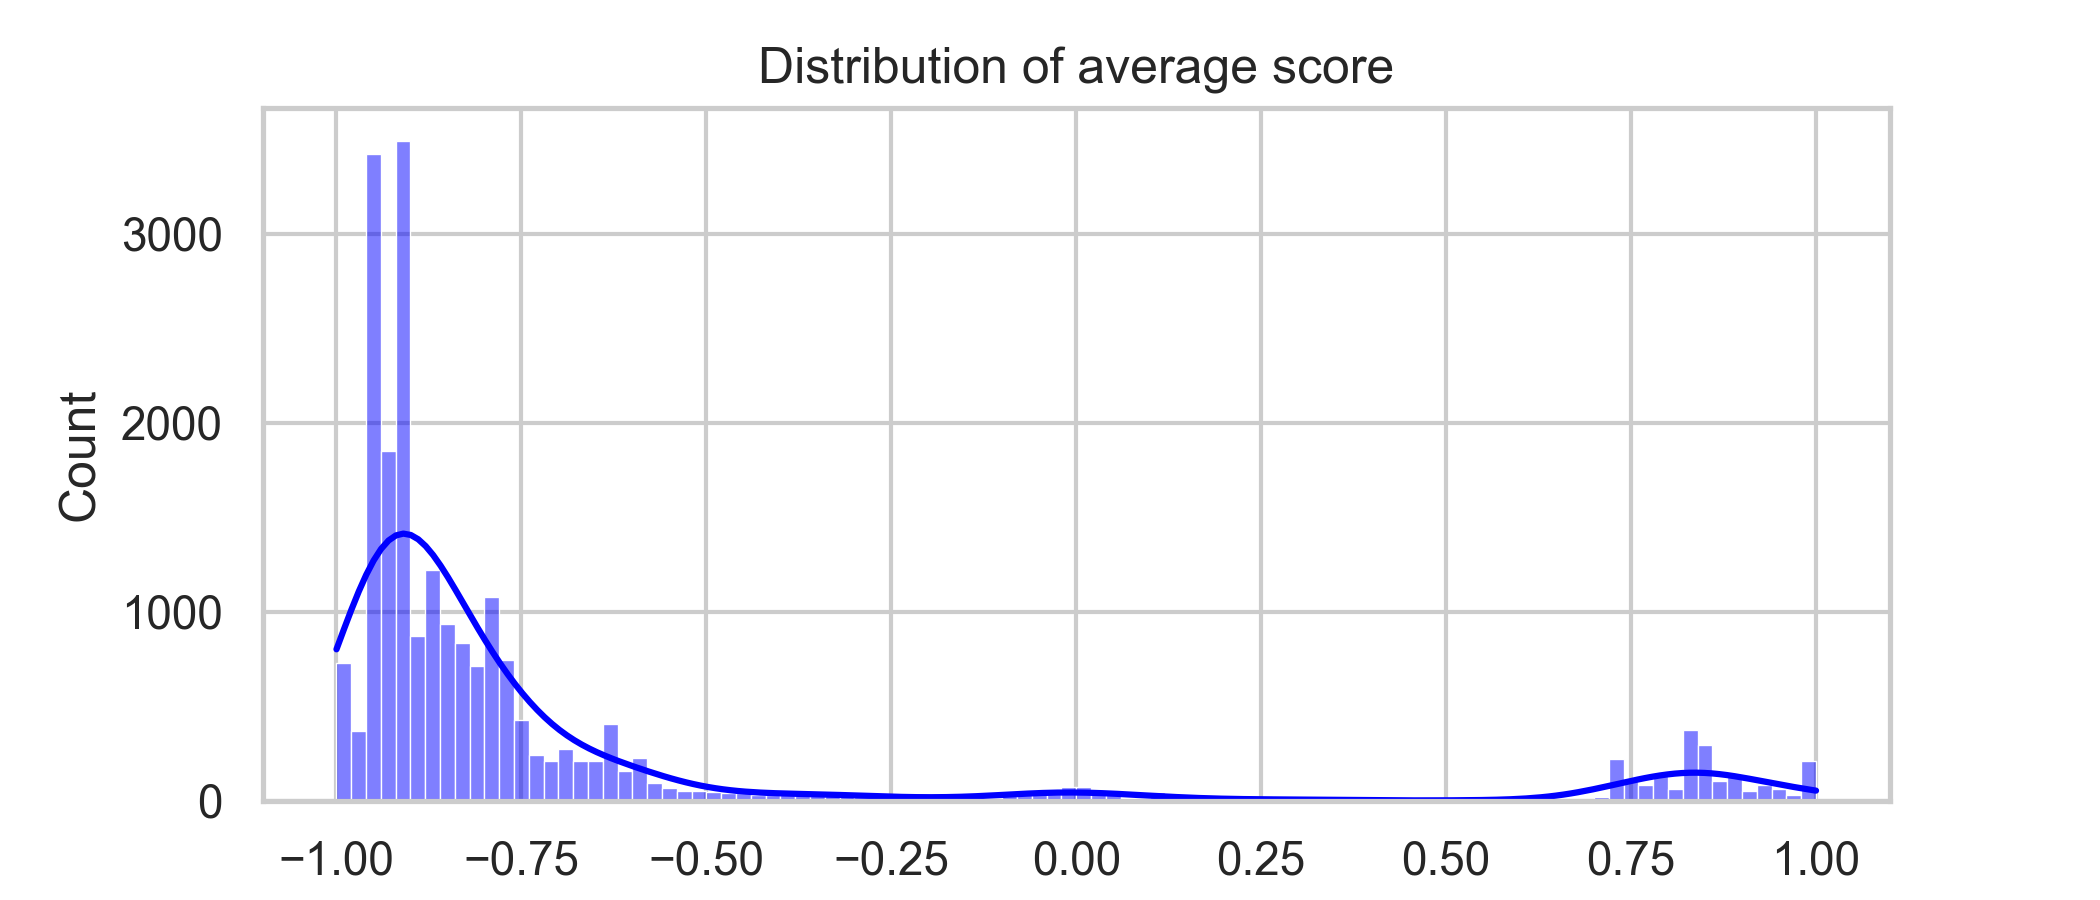
\includegraphics[width=0.9\linewidth]{Chapter5//figures/avg_score.png}
    
    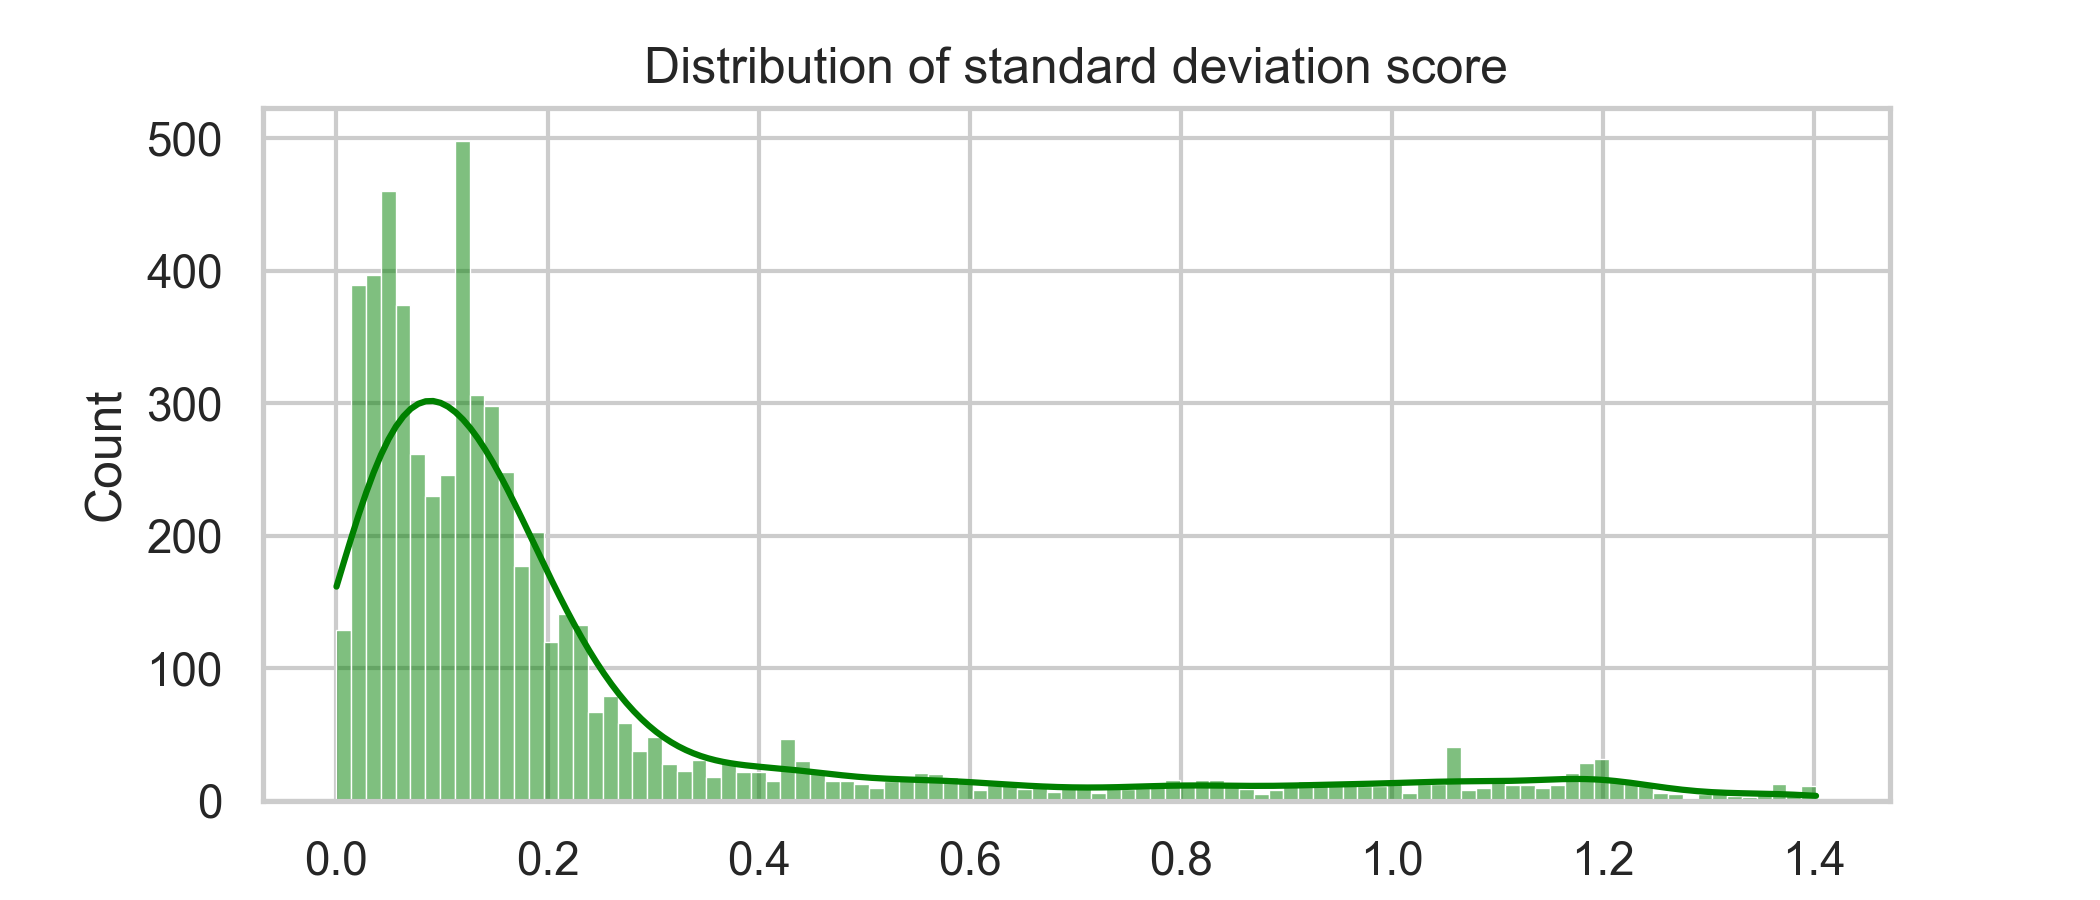
\includegraphics[width=0.9\linewidth]{Chapter5//figures/std_score.png}
    \caption{Enter Caption}
    \label{fig:std_avg}
\end{figure}



\section{RQ4 Polarization of experts vs know-it-all }
Out of the 22k users 16k are present only in one topics, 6k in more then one of which 3k only in 2 topics. \ref{fig:monopoli} do not show a difference in the ideology score between mono and poli user, to compute it we had to get the abs of the ideology so we do not have the problem of getting some mean around 0 

\begin{figure}
    \centering
    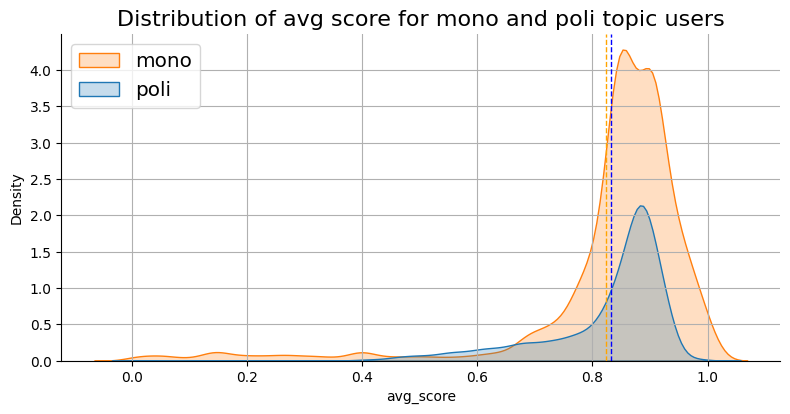
\includegraphics[width=0.8\linewidth]{Chapter5//figures/monopoli_score.png}
    \caption{Enter Caption}
    \label{fig:monopoli}
\end{figure}


\chapter{Results}
%\chapter{Conclusions}




% ********************************** Back Matter *******************************
% Backmatter should be commented out, if you are using appendices after References
%\backmatter

% ********************************** Bibliography ******************************
\begin{spacing}{0.9}

% To use the conventional natbib style referencing
% Bibliography style previews: http://nodonn.tipido.net/bibstyle.php
% Reference styles: http://sites.stat.psu.edu/~surajit/present/bib.htm

\bibliographystyle{plain}
%\bibliographystyle{unsrt} % Use for unsorted references  
%\bibliographystyle{plainnat} % use this to have URLs listed in References
\cleardoublepage
\bibliography{References/references} % Path to your References.bib file


% If you would like to use BibLaTeX for your references, pass `custombib' as
% an option in the document class. The location of 'reference.bib' should be
% specified in the preamble.tex file in the custombib section.
% Comment out the lines related to natbib above and uncomment the following line.

%\printbibliography[heading=bibintoc, title={References}]


\end{spacing}

% ********************************** Appendices ********************************

\begin{appendices} % Using appendices environment for more functunality

%%!TEX root = ../thesis.tex
% ******************************* Thesis Appendix A ****************************
\chapter{How to install \LaTeX} 

\section*{Windows OS}

\subsection*{TeXLive package - full version}
\begin{enumerate}
\item	Download the TeXLive ISO (2.2GB) from\\
\href{https://www.tug.org/texlive/}{https://www.tug.org/texlive/}
\item	Download WinCDEmu (if you don't have a virtual drive) from \\
\href{http://wincdemu.sysprogs.org/download/}
{http://wincdemu.sysprogs.org/download/}
\item	To install Windows CD Emulator follow the instructions at\\
\href{http://wincdemu.sysprogs.org/tutorials/install/}
{http://wincdemu.sysprogs.org/tutorials/install/}
\item	Right click the iso and mount it using the WinCDEmu as shown in \\
\href{http://wincdemu.sysprogs.org/tutorials/mount/}{
http://wincdemu.sysprogs.org/tutorials/mount/}
\item	Open your virtual drive and run setup.pl
\end{enumerate}

or

\subsection*{Basic MikTeX - \TeX~ distribution}
\begin{enumerate}
\item	Download Basic-MiK\TeX (32bit or 64bit) from\\
\href{http://miktex.org/download}{http://miktex.org/download}
\item	Run the installer 
\item	To add a new package go to Start >> All Programs >> MikTex >> Maintenance (Admin) and choose Package Manager
\item	Select or search for packages to install
\end{enumerate}

\subsection*{TexStudio - \TeX~ editor}
\begin{enumerate}
\item	Download TexStudio from\\
\href{http://texstudio.sourceforge.net/\#downloads}
{http://texstudio.sourceforge.net/\#downloads} 
\item	Run the installer
\end{enumerate}

\section*{Mac OS X}
\subsection*{MacTeX - \TeX~ distribution}
\begin{enumerate}
\item	Download the file from\\
\href{https://www.tug.org/mactex/}{https://www.tug.org/mactex/}
\item	Extract and double click to run the installer. It does the entire configuration, sit back and relax.
\end{enumerate}

\subsection*{TexStudio - \TeX~ editor}
\begin{enumerate}
\item	Download TexStudio from\\
\href{http://texstudio.sourceforge.net/\#downloads}
{http://texstudio.sourceforge.net/\#downloads} 
\item	Extract and Start
\end{enumerate}


\section*{Unix/Linux}
\subsection*{TeXLive - \TeX~ distribution}
\subsubsection*{Getting the distribution:}
\begin{enumerate}
\item	TexLive can be downloaded from\\
\href{http://www.tug.org/texlive/acquire-netinstall.html}
{http://www.tug.org/texlive/acquire-netinstall.html}.
\item	TexLive is provided by most operating system you can use (rpm,apt-get or yum) to get TexLive distributions
\end{enumerate}

\subsubsection*{Installation}
\begin{enumerate}
\item	Mount the ISO file in the mnt directory
\begin{verbatim}
mount -t iso9660 -o ro,loop,noauto /your/texlive####.iso /mnt
\end{verbatim}

\item	Install wget on your OS (use rpm, apt-get or yum install)
\item	Run the installer script install-tl.
\begin{verbatim}
	cd /your/download/directory
	./install-tl
\end{verbatim}
\item	Enter command `i' for installation

\item	Post-Installation configuration:\\
\href{http://www.tug.org/texlive/doc/texlive-en/texlive-en.html\#x1-320003.4.1}
{http://www.tug.org/texlive/doc/texlive-en/texlive-en.html\#x1-320003.4.1} 
\item	Set the path for the directory of TexLive binaries in your .bashrc file
\end{enumerate}

\subsubsection*{For 32bit OS}
For Bourne-compatible shells such as bash, and using Intel x86 GNU/Linux and a default directory setup as an example, the file to edit might be \begin{verbatim}
edit $~/.bashrc file and add following lines
PATH=/usr/local/texlive/2011/bin/i386-linux:$PATH; 
export PATH 
MANPATH=/usr/local/texlive/2011/texmf/doc/man:$MANPATH;
export MANPATH 
INFOPATH=/usr/local/texlive/2011/texmf/doc/info:$INFOPATH;
export INFOPATH
\end{verbatim}
\subsubsection*{For 64bit OS}
\begin{verbatim}
edit $~/.bashrc file and add following lines
PATH=/usr/local/texlive/2011/bin/x86_64-linux:$PATH;
export PATH 
MANPATH=/usr/local/texlive/2011/texmf/doc/man:$MANPATH;
export MANPATH 
INFOPATH=/usr/local/texlive/2011/texmf/doc/info:$INFOPATH;
export INFOPATH

\end{verbatim}



%\subsection{Installing directly using Linux packages} 
\subsubsection*{Fedora/RedHat/CentOS:}
\begin{verbatim} 
sudo yum install texlive 
sudo yum install psutils 
\end{verbatim}


\subsubsection*{SUSE:}
\begin{verbatim}
sudo zypper install texlive
\end{verbatim}


\subsubsection*{Debian/Ubuntu:}
\begin{verbatim} 
sudo apt-get install texlive texlive-latex-extra 
sudo apt-get install psutils
\end{verbatim}

%%!TEX root = ../thesis.tex
% ******************************* Thesis Appendix B ********************************

\chapter{Installing the CUED class file}

\LaTeX.cls files can be accessed system-wide when they are placed in the
<texmf>/tex/latex directory, where <texmf> is the root directory of the user’s \TeX installation. On systems that have a local texmf tree (<texmflocal>), which
may be named ``texmf-local'' or ``localtexmf'', it may be advisable to install packages in <texmflocal>, rather than <texmf> as the contents of the former, unlike that of the latter, are preserved after the \LaTeX system is reinstalled and/or upgraded.

It is recommended that the user create a subdirectory <texmf>/tex/latex/CUED for all CUED related \LaTeX class and package files. On some \LaTeX systems, the directory look-up tables will need to be refreshed after making additions or deletions to the system files. For \TeX Live systems this is accomplished via executing ``texhash'' as root. MIK\TeX users can run ``initexmf -u'' to accomplish the same thing.

Users not willing or able to install the files system-wide can install them in their personal directories, but will then have to provide the path (full or relative) in addition to the filename when referring to them in \LaTeX.

\end{appendices}

% *************************************** Index ********************************
\printthesisindex % If index is present

\end{document}
